
%\chapter{由粗到细求解时-空关键帧约束的交通仿真}
\chapter{基于时-空关键帧控制的交通仿真}
\label{chapter:keyframe}


%随着自动驾驶、城市规划、影视游戏等领域的蓬勃发展,交通仿真技术也越来越受人们的关注,因此一个能产生高保真结果的可靠交通仿真器也变得越发的有价值。

%虽然现有的各类交通仿真器~\cite{krajzewicz2002sumo, adnan2016simmobility, fellendorf1994vissim, dosovitskiy2017carla}可以模拟逼真的交通流,但是对车流中某一个个体的行为进行约束控制的工作却鲜有被提出。假设用户想要仿真某一个预定义的场景,或是让车辆表现出预设的运动行为,用户需要反复试错不同的仿真器参数并运行仿真程序使结果逼近预期——这是一个十分繁琐且耗时的过程。交互式编辑技术在人群动画领域被引入解决相似的问题~\cite{kim2014interactive, zhang2020crowd, montana2017sketching},用于让仿真过程变得更直观可控,降低生成特定结果的人力成本,提高动画制作效率。最近,研究者们提出了TraEDITS(章节~\ref{chapter:traedits})用于提高交通仿真中预期车辆行为的生成效率。但是,该框架并不支持用户在时-空多维度上对车辆行为进行约束,例如让某一特定车辆在规定的时刻到达一个特定的位置,这很大程度上限制了用户对车辆运动控制的灵活性。早期的交通流重建工作~\cite{van2007kinodynamic, sewall2010virtualized}提供了一种通过在离散的状态-时间空间中求解约束,让车辆运动在时间和空间上同时满足用户预期的有效方法。但使用该方法会降低生成结果的质量,如存在不连续或跳变的轨迹点,且该方法的计算成本巨大,导致其难以被扩展或集成到其他应用中。

在结合了交互式编辑技术后,TraEDITS框架(第~\ref{chapter:traedits}章)能够让用户通过仿真过程中实时干预个体的行为,如修改个体的系数、实时点击关键点位以生成自定义的参考路径来引导车辆运动等,实现了可视化交通仿真中个体行为多样性和用户预期数据定制化效率的双重提高,引入了包含U型掉头、跨多车道变道和借道超车等非常规驾驶行为的边缘交通案例。但是,TraEDITS的交互逻辑并不支持用户在时-空多维度上约束个体的行为,这很大程度上限制了用户对车辆运动控制的灵活程度——假如用户需要创造出如变道后闯红灯的交通场景,或让某一特定车辆在规定的时刻到达一个特定的位置,仍旧需要反复地调试个体的预期速度参数、手动规划合适的参考路径来实现。


早期的交通流重建工作~\cite{van2007kinodynamic, sewall2010virtualized}提供了一种通过在离散的状态-时间空间中求解约束,让车辆运动在时间和空间上同时满足用户预期的有效方法。但使用该方法会降低生成结果的质量,如存在不连续或跳变的轨迹点,且该方法的计算成本巨大,导致其难以被扩展或集成到其他应用中。受Heter-sim~\cite{ren2019heter}工作启发,TraEDITS框架集成了一个基于优化的交通仿真模块,利用真实获取的交通轨迹数据提高生成结果的可靠性。但想要在基于优化的仿真过程添加额外的约束,再利用数值优化的方法去求解,存在一个根本的挑战:仿真过程的不可微性,导致基于梯度的约束求解方法在本质上不适用。值得注意的是,在人群动画中广泛应用的社会力模型近期在交通仿真中也展现出了巨大的潜力,一个统一的社会力模型~\cite{chao2019force}与简化的社会力模型(章节~\ref{chapter:simplified})相继被提出应用于多种类智能体的混合交通仿真中。由于智能体的状态更新使用可导的表达式进行了显式地建模,所以基于社会力模型使用数值优化来求解约束具有可行性。但是,现有的基于社会力的交通仿真方法只能提供包含直道的简单仿真场景,且车辆只能严格在车道的中心线附近行驶,不能满足用户任意编辑的需求。

为了将时-空约束与基于社会力模型的交通仿真动画相结合,我们引入了关键帧这一在物理仿真中能有效控制生成结果的概念,将用户的交互式编辑操作从TraEDITS中点击关键位置变为点击关键帧。伴随法(Adjoint Method)作为基于梯度下降求解最优化控制的经典方法,已经成功应用在了如流体模拟~\cite{mcnamara2004fluid}和通用粒子系统动画~\cite{wojtan2006keyframe}的关键帧约束求解。但是伴随法优化过程高度依赖于初始化设置,如果待优化参数的初始值与最优值相差太大,极有可能降低梯度下降的收敛速度,甚至导致其最终发散。

综上所述,本章提出了一个新颖的交互式交通仿真方法,允许用户在仿真进行时使用时-空关键帧控制车辆行为、编辑车辆轨迹。延续了TraEDITS框架的思想,我们基于社会力模型并使用Cartesian坐标系和Frenet坐标系混合表示和更新车辆状态,使得车辆能够沿着任意参考路径行驶而非强行限制在车道中心线附近;与TraEDITS框架不同的是,我们将交通仿真部分替换为了基于社会力的仿真模型,以发挥其可微的特性。为了更高效地求解关键帧约束,我们提出了一个由粗到细(Coarse-to-Fine)的优化过程,保证梯度下降快速稳定收敛的同时生成的交通轨迹足够平滑且合理。本方法的主要贡献如下:

\begin{itemize}
    \item 提出了一个允许用户使用时-空关键帧控制的交通轨迹编辑方法,能够快捷方便地生成满足用户要求的真实交通轨迹。

    \item 提出了一个基于力的个体运动控制模型,能将车辆运动从静态车道解耦表示和计算,并结合用户输入的关键帧约束在复杂的道路场景中生成多样的交互行为。

    \item 提出了一个由粗到细求解时-空关键帧约束的优化过程,将状态-时间空间搜索的结果与伴随法相结合,保证梯度下降快速稳定收敛的同时能够生成足够平滑且合理的交通轨迹。
    
\end{itemize}



\section{方法概述}

图~\ref{fig:keyframe_overview}展示了使用时-空关键帧控制的交通仿真和由粗到细求解关键帧约束的流程:
\begin{figure}[!h]
%\setlength{\abovecaptionskip}{-0.1cm} 
%\setlength{\belowcaptionskip}{-0.45cm}
\centering
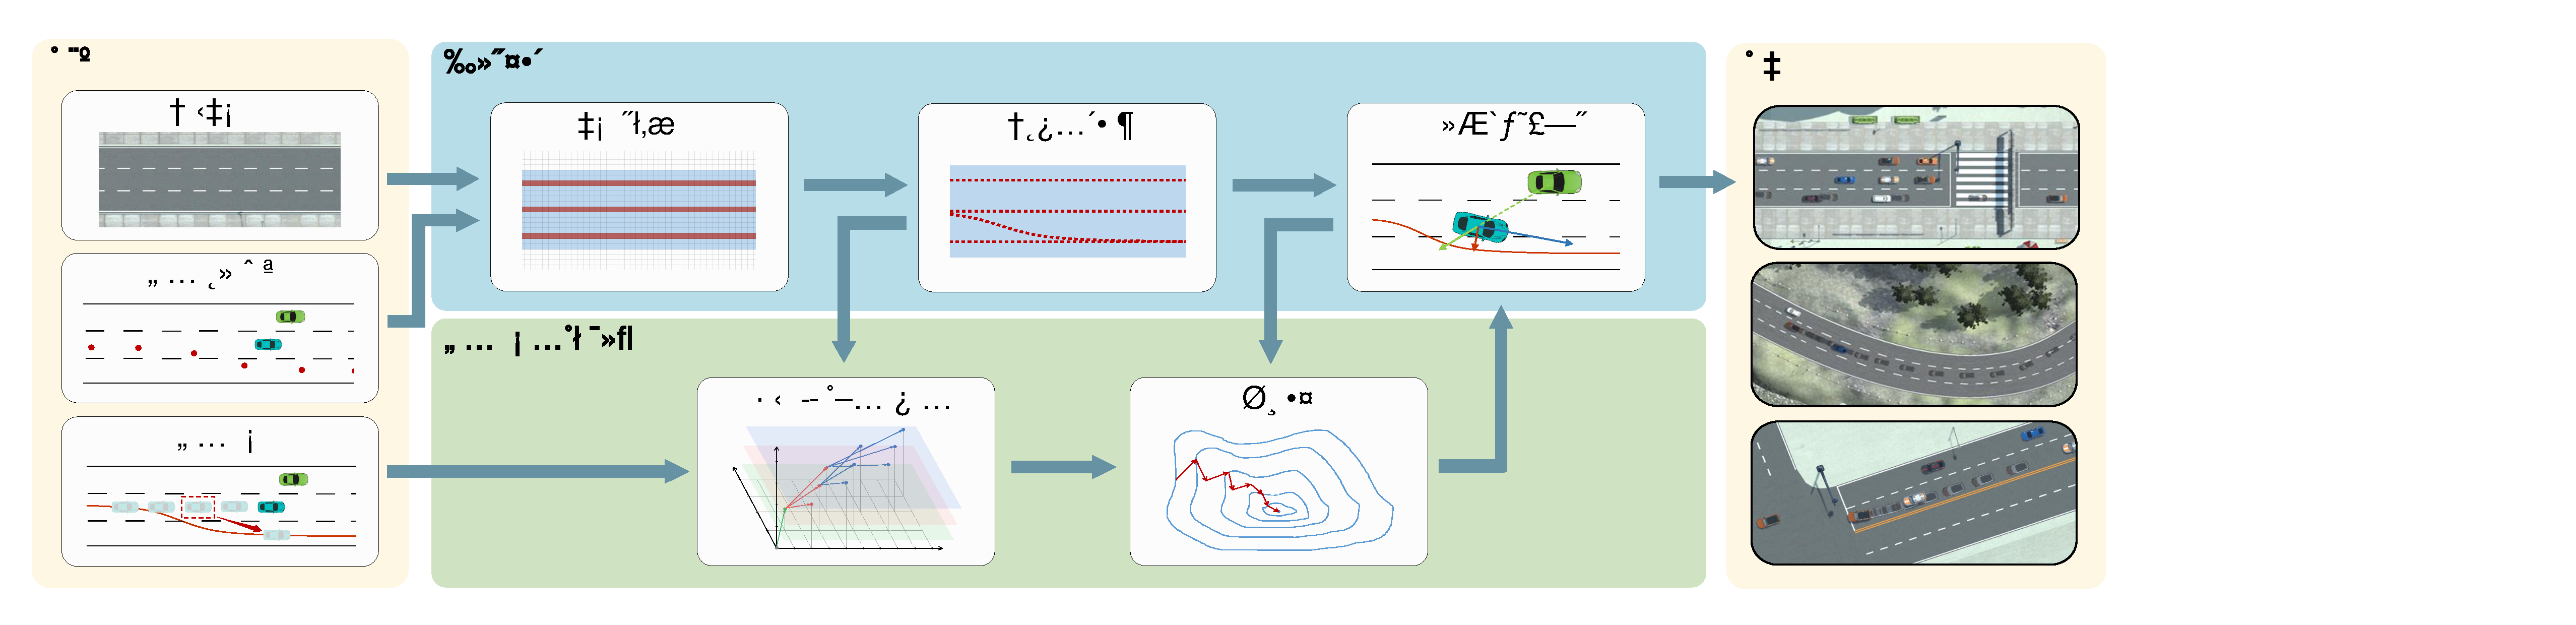
\includegraphics[width=\textwidth]{figure/keyframe/framework_v3.1_cn.pdf}
%\caption[时-空关键帧控制的交通仿真流程示意图]{
%时-空关键帧控制的交通仿真流程示意图。在离散化给定场景后,我们使用用户指定的关键点生成自定义的参考路径,并基于社会力模型沿着参考路径更新车辆状态和运动。在指定关键帧后,粗粒度的状态-时间搜索结果与细粒度的伴随法优化将结合,以高效地生成平滑且满足关键帧约束的交通轨迹。}
\caption[时-空关键帧控制的交通仿真流程图]{
时-空关键帧控制的交通仿真流程图
}
\label{fig:keyframe_overview}
\end{figure}

我们首先简述了场景空间和车辆状态的表示方法,以及参考路径规划的过程(章节~\ref{section:keyframe_represent&plan});基于该表示方法,进一步提出了可微的交通仿真社会力模型,包含车辆的自驱动力、路径保持力与碰撞避免力(章节~\ref{section:keyframe_forcesimulate})。为了满足关键帧的时-空约束,我们提出了一个由粗到细的优化过程,先在状态-时间空间搜索粗粒度的轨迹(章节~\ref{section:keyframe_coarseopt}),从粗粒度的轨迹中提取出信息用以初始化伴随法进行细粒度的优化(章节~\ref{section:keyframe_fineopt})以得到平滑且合理的结果。在实验部分,我们展示了使用时-空关键帧控制的交通轨迹案例(章节~\ref{section:keyframe_cases}),基于对比试验展示了我们的方法的运行效率(章节~\ref{section:keyframe_performance})。特别地,我们还展示了部分经由本方法生成的失败案例,以及使用本方法进行迭代式修复后对应的改善案例(章节~\ref{section:keyframe_failure})。





\section{基于可微社会力模型和参考路径坐标系的交通仿真}


\subsection{场景表示与参考路径规划}
\label{section:keyframe_represent&plan}

我们在Cartesian坐标系和Frenet坐标系中同时表示车辆的状态与更新其运动。Frenet坐标记为$[s, d]$,其中$s$表示车辆从道路起点开始沿着道路的纵向位移距离,$d$表示车辆偏移当前道路的横向位移距离。我们记$\textbf{\emph{p}}=[x, y]$, $\hat{\textbf{\emph{p}}}=[s, d]$, $\textbf{\emph{v}}=[v^x, v^y]$和$\hat{\textbf{\emph{v}}}=[v^s, v^d]$分别表示车辆在Cartesian坐标系和Frenet坐标系中的位置和速度。相似地,我们使记$\textbf{\emph{f}}=[f^x, f^y]$和$\hat{\textbf{\emph{f}}}=[f^s, f^d]$或其他相同上标的变量,分别表示在这两个坐标系中的力或其他车辆属性。

与TraEDITS工作相似,我们使用同样的流程将整个场景离散化成二维网格,并基于胶囊状对车道几何进行近似,从而将整个场景的车道信息编码到网格单元内(章节~\ref{section:traedits_discretize})。对于一个给定的场景,其中包含的车道信息是确定的,因此我们初始化整个场景的参考路径为:
\begin{equation}
\setlength\abovedisplayskip{6pt}
\setlength\belowdisplayskip{6pt}
\label{eq:keyframe_initpath}
\begin{aligned}
    &\mathcal{P}^* = {\mathcal{P}^*_{topo}}\cup{\mathcal{P}^*_{user}}, \\
    &\mathcal{P}^*_{topo} = DFS\left(\mathcal{L}^*\right), \\
    &\mathcal{P}^*_{user} = \varnothing,
\end{aligned}
\end{equation}
其中$\mathcal{P}^*$表示所有参考路径的集合,包含车道网络的拓扑关系所决定的参考路径$\mathcal{P}^*_{topo}$与用户自定义的参考路径$\mathcal{P}^*_{user}$。$\mathcal{P}^*_{topo}$则由深度优先搜索车道网络集合$\mathcal{L}^*$得到,其中每一条参考路径表示从一条无入车道的车道起点到一条无出车道的车道终点的唯一连接。

用户在场景中点击一系列关键点后,这些关键点被映射到对应的网格单元中,并使用改进的A*启发式路径搜索算法生成新的路径,新的启发式函数为:
\begin{equation}
\setlength\abovedisplayskip{6pt}
\setlength\belowdisplayskip{6pt}
\label{eq:keyframe_heuristic}
    h(\textbf{n}) = || \textbf{n} - \textbf{n}_{goal} || + \mu_a  \cdot e^{\left( \mu_b \cdot \rm{sign} \right)},
\end{equation}
其中$|| \textbf{\emph{n}} - \textbf{n}_{goal} ||$表示当前网格单元与目标网格单元之间的欧氏距离,$\rm{sign}\in[0,1,2]$中$0$表示当前网格单元为不可行驶区域,$1$表示为可行驶区域,$2$表示车道中心线区域,$\mu_a$,$\mu_b$是两个可调节的系数。我们使用降采样、高斯滤波和样条插值的方法对规划得到粗糙的参考路径进行后处理,使其最终足够平滑以供车辆选择跟随,记为$\mathcal{P}^*_{user} = \mathcal{P}^*_{user} \cup [\mathcal{P}]$。


\subsection{车辆受力分析}
\label{section:keyframe_forcesimulate}

在得到了不同的参考路径之后,我们将基于社会力模型沿着参考路径更新车辆的状态和运动。我们考虑三个对车辆运动息息相关的因素:运动目标,环境与周围邻车。我们记一辆车在$t$时刻下的状态为$[\hat{\textbf{\emph{v}}}_t, \hat{\textbf{\emph{p}}}_t, \textbf{\emph{v}}_t, \textbf{\emph{p}}_t, \theta_t, \hat{\textbf{\emph{v}}}_{o,t}, \mathcal{P}_{k}]$,其中$\hat{\textbf{\emph{v}}}_t, \textbf{\emph{v}}_t\in\mathbb{R}^2$分别表示车辆在Frenet坐标系和Cartesian坐标系中的速度,$\hat{\textbf{\emph{p}}}_t$,  $\textbf{\emph{p}}_t\in\mathbb{R}^2$分别表示车辆在Frenet坐标系和Cartesian坐标系中的位置,$\theta_t\in\mathbb{R}$为欧拉角表示的车辆朝向,$\hat{\textbf{\emph{v}}}_{o,t}\in\mathbb{R}^2$表示车辆在未受阻挡时的预期行驶速度,$\mathcal{P}_{k}\in\mathcal{P}^*$表示车辆当前跟随的参考路径。车辆在Cartesian坐标系和Frenet坐标系中的属性可以通过参考路径的三次样条函数$S_k$转变得到。车辆的状态变化表示为:
\begin{equation}
\setlength\abovedisplayskip{6pt}
\setlength\belowdisplayskip{6pt}
\label{eq:keyframe_dynamics}
\begin{aligned}
    %& \hat{\textbf{\emph{f}}}_{t} = \hat{\textbf{\emph{f}}}_{o,t} + \hat{\textbf{\emph{f}}}_{k,t} + \sum_{j\in \mathcal{N}_{t}}\hat{\textbf{\emph{f}}}_{j,t}, \\
    & \hat{\textbf{\emph{f}}}_{t} = \hat{\textbf{\emph{f}}}_{o,t} + \hat{\textbf{\emph{f}}}_{k,t} + S_k \left( \sum_{j\in \mathcal{N}_{t}}{\textbf{\emph{f}}}_{j,t} \right), \\
    & \hat{\textbf{\emph{v}}}_{t+1} = \hat{\textbf{\emph{v}}}_t + \frac{\hat{\textbf{\emph{f}}}_{t}}{m} \cdot \Delta{t}, \\
    & \hat{\textbf{\emph{p}}}_{t+1} = \hat{\textbf{\emph{p}}}_t + \hat{\textbf{\emph{v}}}_{t+1} \cdot \Delta{t}, \\
    [ & \textbf{\emph{v}}_{t+1}, \textbf{\emph{p}}_{t+1}, \theta_{t+1}] = S_k\left( \hat{\textbf{\emph{p}}}_{t+1} \right), 
\end{aligned}
\end{equation}
其中$m$表示车辆质量,$\hat{\textbf{\emph{f}}}_{t}$表示在Frenet坐标系下当前时刻车辆所受到的合力,由自驱动力$\hat{\textbf{\emph{f}}}_{o,t}$,当前参考路径$\mathcal{P}_k$施加的路径保持力$\hat{\textbf{\emph{f}}}_{k,t}$,以及所有在其邻车集合$\mathcal{N}_{t}$中的车辆$j$施加的碰撞避免力求和得到。需要注意的是,碰撞避免力需要在Cartesian坐标系中求得后进一步转换到Frenet坐标系中才能计算合力。经过计算得到合力后,我们可以更新Frenet坐标系下的速度和位置,其余车辆属性亦可以通过参考路径的样条插值函数转换得到。另外,$\Delta{t}$表示的是仿真方法中使用的时间步长,需要与后续优化过程中的时间步长作区分。

\textbf{自驱动力:}我们假设每一辆车在无前车阻挡的情况下期望以一个特定的速度在道路上行驶。与先前基于社会力的交通仿真方法~\cite{chao2019force, chao2021calibrated}不同,我们将车辆的自驱动力定义为:
\begin{equation}
\setlength\abovedisplayskip{6pt}
\setlength\belowdisplayskip{6pt}
\label{eq:keyframe_selfmotivate}
    \hat{\textbf{\emph{f}}}_{o,t} = \omega_o m \left( \frac{2}{1+e^{\hat{\textbf{\emph{v}}}_{o,t} - \hat{\textbf{\emph{v}}}_{t}}} - 1 \right) \hat{\textbf{\emph{a}}},
\end{equation}
其中$\omega_o$是求和权重,$\hat{\textbf{\emph{a}}}$是车辆在Frenet坐标系中的最大加速度。经过这样建模,车辆能够在运动过程中倾向于逐渐加速至预期速度$\hat{\textbf{\emph{v}}}_{o,t}$,同时又能保证表达式在其定义域上是易于求导的。

\textbf{路径保持力:}通常情况下,驾驶员为了保证安全和遵守交通规则,都倾向于保持在车道的中心线附近行驶。在本方法中,我们将连续车道的中心线组合亦视为一条参考路径,因此车道保持行为可等效视为路径保持。我们定义路径保持力为参考路径对车辆的吸引力:
\begin{equation}
\setlength\abovedisplayskip{6pt}
\setlength\belowdisplayskip{6pt}
\label{eq:keyframe_pathkeep}
    %\hat{\textbf{\emph{f}}}_{k} = \omega_{k} \left| d \right|,
    \hat{\textbf{\emph{f}}}_{k} = 
    \left\{
        \begin{array}{lr}
        \omega_{k} \left| d_t \right| \textbf{\emph{u}}_k, & \left| d_t \right| \geq \frac{1}{2}(w_l - w_v) \\
        \textbf{\emph{0}}, & otherwise
        \end{array}, 
    \right.
\end{equation}
其中$\omega_k$是求和权重,$d_t\in\hat{\textbf{\emph{p}}}_t$是车辆当前偏离路径的横向距离,$\textbf{\emph{u}}_k$是从车辆当前位置指向参考路径上最近点的单位向量,$w_l$和$w_v$分别使车道和车辆的宽度。如表达式~\ref{eq:keyframe_pathkeep}所示,路径保持力只在车辆相对参考路径的偏移距离超过一定阈值之后才会生效,这样设计的目的是保证车辆不会过度偏离参考路径,同时防止车辆因微小偏移而在路径周围来回震荡。

\textbf{碰撞避免力:}车辆需要避免与过于接近的邻车发生碰撞,因此我们将这样的车辆与其周围邻车之间的相互影响建模为点到点的排斥力。一辆车与其邻车$j$的碰撞避免力定义为:
\begin{equation}
\setlength\abovedisplayskip{6pt}
\setlength\belowdisplayskip{6pt}
\label{eq:keyframe_collisionavoid}
\begin{aligned}
    & {\textbf{\emph{f}}}_{j} = \omega_c \frac{a  \cdot b }{\left(1+c||\textbf{\emph{p}}_{j,t} - \textbf{\emph{p}}_t||  \right)^2}\textbf{\emph{u}}_c, \\
    & a = \left\{
        \begin{array}{lr}
        \rm{cos} \phi, & \phi \leq \frac{\pi}{4} \\
        0, & otherwise
        \end{array}, 
    \right. \\
    & b = s_0 + ||\textbf{\emph{v}}_t || T_0 + \frac{||\textbf{\emph{v}}_t||\cdot || \textbf{\emph{v}}_{j,t} - \textbf{\emph{v}}_t ||}{2||\hat{\textbf{\emph{a}}}||}, \\
    & c = \frac{1}{s_0},
\end{aligned}
\end{equation}
其中$\omega_c$是求和权重,$a$是视角系数,$b$和$c$是使用车辆物理属性参数化后得到的系数,参数化过程受Intelligent Driver Model (IDM)模型~\cite{treiber2000congested-idm}的启发。$\textbf{\emph{u}}_c$是从邻车$j$指向目标车辆的单位向量,$\phi$是目标车辆的运动方向与目标车辆指向邻车$j$的方向的夹角,$\textbf{\emph{v}}_{j,t}$和$\textbf{\emph{p}}_{j,t}$表示邻车$j$在Cartesian坐标系中的速度和位置。$s_0$和$T_0$表示车辆的安全跟车距离与制动所需要的反应时间,二者均为预设常数。邻车集合$\mathcal{N}_t$包含了一定范围内可能对目标车辆产生影响的所有其他车辆,我们利用离散化场景时生成的网格结构加速领域搜索和集合的实时更新,搜索邻车的范围在我们的实验中设置为$100\times100$网格单元。


\section{由粗到细的时-空关键帧优化}

为了满足进一步使用时-空关键帧对基于社会力模型的交通仿真进行控制,我们使用已经被证明有效的伴随法来求解关键帧的约束。通过伴随法,我们可以找到一系列最优行驶速度和对应所要施加的控制力大小,使车辆的运动最终满足关键帧的时-空约束。然而,伴随法基于梯度下降进行优化,而基于梯度学习的优化方法对待优化参数的初始值设定非常敏感。假如初始化数值选取不佳,会降低梯度下降的收敛速度,甚至最终导致梯度的发散。因此,我们在使用伴随法求解关键帧之前,先在车辆的状态-时间空间中进行一个粗粒度的搜索,并从这个粗粒度的轨迹中提取对应的信息来初始化伴随法的待优化参数,从而保证梯度下降的快速稳定收敛。算法~\ref{alg:keyframe_optimization}中展示了我们提出的由粗到细求解关键帧约束的优化方法,接下来我们会进一步介绍其中的细节。

\begin{algorithm}[!tbh]
%\setlength{\abovecaptionskip}{-0.05cm} 
\setlength{\belowdisplayskip}{-0.25cm}
\setstretch{1.2}
\caption{由粗到细求解时-空关键帧约束}
\label{alg:keyframe_optimization}
\begin{algorithmic}[1]

\REQUIRE ~~\\ %算法的输入参数:Input
    车辆沿其参考路径构建的状态-时间有向图; \\
    包含$K$个关键帧的集合 $Q= [\Tilde{\textbf{\emph{q}}}_0, \Tilde{\textbf{\emph{q}}}_1, ..., \Tilde{\textbf{\emph{q}}}_K]$; \\
    伴随法的最大迭代次数$N$; \\
    Adam优化器的学习率$\alpha$和指数衰减率 $\beta_0$, $\beta_1$; \\
\ENSURE ~~\\ %算法的输出:Output
    受关键帧约束生成的轨迹$\mathcal{T}$; \\~\\

\STATE 初始化沿轨迹的预期速度 $V \Leftarrow \varnothing$, 对应的社会力 $F \Leftarrow \varnothing$; 
\FOR{$i=0 $ to $K-1$}
    \STATE 状态-时间起始节点$[s_{start}, v^s_{start}, t_{start}] \Leftarrow \Tilde{\textbf{\emph{q}}}_i$;
    \STATE 状态-时间目标节点$[s_{goal}, v^s_{goal}, t_{goal}] \Leftarrow \Tilde{\textbf{\emph{q}}}_{i+1}$;
    \STATE 使用A*算法在状态-时间有向图中寻找一条粗粒度的轨迹 $\mathcal{T}_c \Leftarrow \mathcal{A}^*([s_{start}, v^s_{start}, t_{start}], [s_{goal}, v^s_{goal}, t_{goal}])$;
    \STATE 提取当前粗粒度轨迹 $\mathcal{T}_c$ 沿途的速度 $V \Leftarrow V\cup[v^s_{o,0}, v^s_{o,1},...]$;
\ENDFOR

\STATE 对齐预期速度$V$集合的帧数;

\FOR{$i=0$ to $N-1$}
    \STATE 计算预期速度对应的社会力集合 $F \Leftarrow V$;
    %\STATE Simulate the current whole trajectory $\mathcal{T}_o$ with $F$ using our force-based traffic simulation algorithm;
    \STATE 基于我们的社会力交通仿真模型,使用社会力$F$仿真得到轨迹$\mathcal{T}_o$;
    
    \IF{目标函数损失值下降}
        \STATE 更新轨迹 $\mathcal{T} \Leftarrow \mathcal{T}_o$;
    \ENDIF
    
    \STATE 使用伴随法计算预期速度的梯度 $\nabla{V} \Leftarrow \mathcal{A}djoint(\mathcal{T}_o, V)$;
    
    \STATE 使用Adam优化器进行梯度下降 $V \Leftarrow Adam(\nabla{V}, \alpha,\beta_0,\beta_1)$;
    %\STATE Gradient descent by Adam optimizer, $V \Leftarrow Adam(\nabla{V})$;
\ENDFOR

%\STATE Find a coarse trajectory \\ $T_c = Heuristic Search([s_{start}, v^s_{start}, t_{start}], [s_{goal}, v^s_{goal}, t_{goal}])$;
\RETURN 细粒度轨迹 $\mathcal{T}$;

\end{algorithmic}
\end{algorithm}


% \begin{algorithm}[!tbh]
% %\setlength{\abovecaptionskip}{-0.05cm} 
% \setlength{\belowdisplayskip}{-0.25cm}
% \caption{Coarse-to-Fine Optimization}
% \label{alg:keyframe_optimization}
% \begin{algorithmic}[1]

% \REQUIRE ~~\\ %算法的输入参数:Input
%     State-time graph for a vehicle along its reference path; \\
%     %The start keyframe $[s_{start}, v^s_{start}, t_{start}]$; \\
%     %The goal keyframe $[s_{goal}, v^s_{goal}, t_{goal}]$; \\
%     $K$ setting keyframes $Q= [\Tilde{\textbf{\emph{q}}}_0, \Tilde{\textbf{\emph{q}}}_1, ..., \Tilde{\textbf{\emph{q}}}_K]$; \\
%     The maximum iteration number $N$ for the adjoint method; \\
%     Learning rate $\alpha$, exponential decay rates $\beta_0$, $\beta_1$; \\
% \ENSURE ~~\\ %算法的输出:Output
%     Trajectory $\mathcal{T}$ under keyframes control; \\~\\

% \STATE Initialize controlling desired speeds $V \Leftarrow \varnothing$, controlling forces $F \Leftarrow \varnothing$; 
% \FOR{$i=0 $ to $K-1$}
%     \STATE Start state-time node $[s_{start}, v^s_{start}, t_{start}] \Leftarrow \Tilde{\textbf{\emph{q}}}_i$;
%     \STATE Goal state-time node $[s_{goal}, v^s_{goal}, t_{goal}] \Leftarrow \Tilde{\textbf{\emph{q}}}_{i+1}$;
%     \STATE Find a coarse trajectory in state-time graph with A* algorithm, $\mathcal{T}_c \Leftarrow \mathcal{A}^*([s_{start}, v^s_{start}, t_{start}], [s_{goal}, v^s_{goal}, t_{goal}])$;
%     \STATE Append controlling desired speeds, $V \Leftarrow V\cup[v^s_{o,0}, v^s_{o,1},...]$ extracted from current $\mathcal{T}_c$;
% \ENDFOR

% \STATE Pad controlling  desired speeds $V$;

% \FOR{$i=0$ to $N-1$}
%     \STATE Compute corresponding forces with controlling desired speeds, $F \Leftarrow V$;
%     \STATE Simulate the current whole trajectory $\mathcal{T}_o$ with $F$ using our force-based traffic simulation algorithm;
    
%     \IF{loss decreases}
%         \STATE Update $\mathcal{T} \Leftarrow \mathcal{T}_o$;
%     \ENDIF
    
%     %\STATE Compute gradient of desired speeds using adjoint method, $\nabla{V} \Leftarrow \mathcal{A}djoint(T_o, [\Tilde{\textbf{\emph{n}}}_0, \Tilde{\textbf{\emph{n}}}_1, ..., \Tilde{\textbf{\emph{n}}}_k])$;
%     \STATE Compute gradient of desired speeds using the adjoint method, $\nabla{V} \Leftarrow \mathcal{A}djoint(\mathcal{T}_o, V)$;
    
%     \STATE Gradient descent, $V \Leftarrow Adam(\nabla{V}, \alpha,\beta_0,\beta_1)$;
%     %\STATE Gradient descent by Adam optimizer, $V \Leftarrow Adam(\nabla{V})$;
% \ENDFOR

% %\STATE Find a coarse trajectory \\ $T_c = Heuristic Search([s_{start}, v^s_{start}, t_{start}], [s_{goal}, v^s_{goal}, t_{goal}])$;
% \RETURN Fine trajectory $\mathcal{T}$;

% \end{algorithmic}
% \end{algorithm}





\subsection{粗粒度状态-时间空间搜索}
\label{section:keyframe_coarseopt}

\textbf{状态-时间图构建:}在这个阶段内,我们将一辆汽车的状态空间定义为其完整状态空间的一个子集。重新声明,一辆车的完整状态空间表示为$[\hat{\textbf{\emph{v}}}, \hat{\textbf{\emph{p}}}, \textbf{\emph{v}}, \textbf{\emph{p}}, \theta, \hat{\textbf{\emph{v}}}_{o}, \mathcal{P}_{k}]$,则其沿着当前参考路径方向的状态空间记为$[s, v^s]$,其中$s\in\hat{\textbf{\emph{p}}}$和$v^s\in\hat{\textbf{\emph{v}}}$分别表示Frenet坐标系中沿参考路径方向上的位移分量和速度分量。

我们给定另一个时间步长$\Delta \Tilde{t}$用于构建车辆的状态空间,其数值相较于仿真所用的时间步长更大。假设车辆的实时加速度只能从集合$[-a^s, 0, a^s]$中选取,其中$a^s\in\hat{\textbf{\emph{a}}}$是车辆在Frenet坐标系中的最大加速度沿路径方向的分量。根据表达式~\ref{eq:keyframe_dynamics}所示的车辆状态更新方程,我们可以确定在车辆状态空间中$v^s$轴和$s$轴的采样间隔分别为$\Delta{v^s}=a^s\Delta{\Tilde{t}}$和$\Delta{s}=\frac{1}{2}a^s(\Delta{\Tilde{t}})^2$。因此,对于任意给定的一个状态节点$[s, v^s]$,其在一个时间步长内能够到达的下一个状态节点只有三个,分别为加速后到达的$[s+(2\frac{v^s}{\Delta{v}^s}+1)\Delta{s}, v^s + \Delta{v}^s]$,匀速行驶后到达的$[s+2\frac{v^s}{\Delta{v}^s}\Delta{s}, v^s]$,以及减速后到达的$[s+(2\frac{v^s}{\Delta{v}^s}-1)\Delta{s}, v^s - \Delta{v}^s]$。最终,车辆沿着参考路径的所有状态转移可以表示为一个存在有限个可到达状态节点的有向图。

车辆的状态-时间空间定义为车辆的状态空间中添加时间维度坐标轴而张成的空间。相似地,我们可以在状态-时间空间中建立离散的状态-时间有向图,对于任意给定的状态-时间节点$\Tilde{\textbf{\emph{q}}}=[s, v^s, t]$,其在下一时刻时也只有三个可以到达的状态-时间节点。因此,对于用户给定的时-空关键帧,我们可以将他们映射到对应的状态-时间节点,求解关键帧的约束问题变成了在状态-时间有向图里从起点$[s_{start}, v^s_{start}, t_{start}]$到目标$[s_{goal}, v^s_{goal}, t_{goal}]$寻找一条最优的路径。图~\ref{fig:keyframe_sttspace}中展示了离散的状态-时间空间和构建的有向图。对于任意一个状态-时间节点,其能在下一时刻到达的其他节点用箭头标注出转移方向。不同颜色的平面代表不同的时刻,绿色为$\Delta\Tilde{t}$时刻,红色为$2\Delta\Tilde{t}$时刻,蓝色为$3\Delta\Tilde{t}$时刻,不同的转移箭头也使用了对应的颜色进行标注。

\begin{figure}[!tbh]
%\setlength{\abovecaptionskip}{-0.1cm} 
%\setlength{\belowcaptionskip}{-0.45cm}
\centering
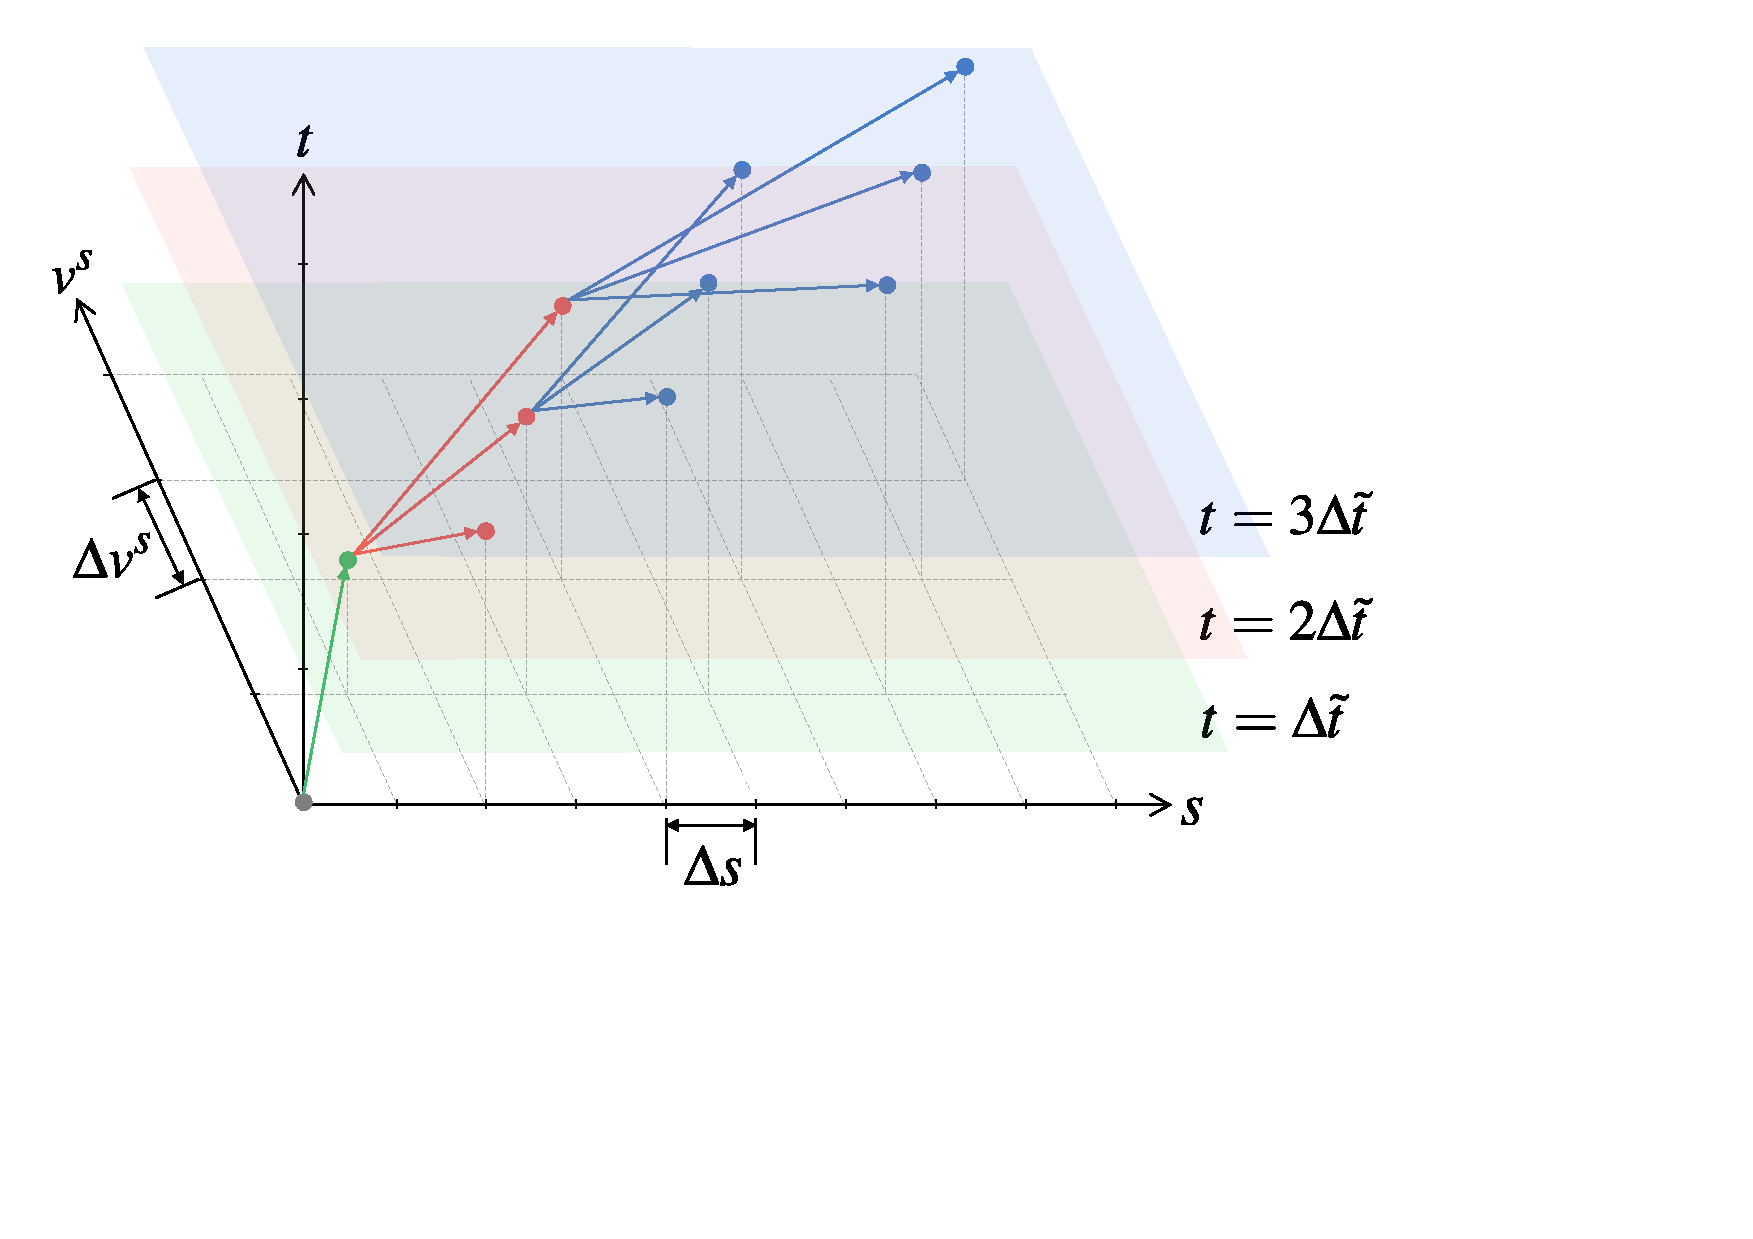
\includegraphics[width=0.65\textwidth]{figure/keyframe/state_time_space.pdf}
%\caption[离散化状态-时间空间与有向图构建]{
%离散的状态-时间空间和有向图构建。对于任意一个状态-时间节点,其能在下一时刻到达的其他节点用箭头标注出转移方向。不同颜色的平面代表不同的时刻,绿色为$\Delta\Tilde{t}$时刻,红色为$2\Delta\Tilde{t}$时刻,蓝色为$3\Delta\Tilde{t}$时刻,不同的转移箭头也使用了对应的颜色进行标注。}
\caption[离散化状态-时间空间与有向图构建]{
离散化状态-时间空间与有向图构建
}
\label{fig:keyframe_sttspace}
\end{figure}

\textbf{粗粒度轨迹搜索:}在状态-时间有向图中寻找一条从起点到终点的轨迹,可以看做在特定的三维解空间中规划一条最优路径。我们同样使用A*路径规划算法进行搜索,搜索中用到的启发式函数定义为:
\begin{equation}
\setlength\abovedisplayskip{10pt}
\setlength\belowdisplayskip{10pt}
\label{eq:keyframe_sttheuristic}
\begin{aligned}
    & \Tilde{h}(\Tilde{\textbf{\emph{q}}}) = \omega_d \Tilde{h}_d(\Tilde{\textbf{\emph{q}}}) + \omega_a \Tilde{h}_a(\Tilde{\textbf{\emph{q}}}), \\
    & \Tilde{h}_d(\Tilde{\textbf{\emph{q}}}) = \sqrt{ | s - s_{goal} |^2 + | v^s - v^s_{goal} |^2 + | t - t_{goal} |^2 },\\
    & \Tilde{h}_a(\Tilde{\textbf{\emph{q}}}) = \frac{|v^s - v^s_{parent}|}{\Delta{\Tilde{t}}} ,\\
\end{aligned}
\end{equation}
其中$\Tilde{h}_d$表示的是当前状态-时间节点与目标点之间的距离,$\Tilde{h}_a$是当前速度相较于上一时刻速度的变化大小,避免使车辆过于频繁地变更速度,$\omega_d$和$\omega_a$是对应的求和权重。

此外,目标车辆以外的其他车辆可以被预处理变成状态-时间空间中的静态障碍物~\cite{sewall2010virtualized}。在A*搜索过程中,被其他车辆占据的状态-时间节点会被标记为不可到达,位移轴超过路径总长度、时间超过最大仿真时间上限的部分也会被禁止探索,避免车辆发生碰撞、驶离车道等非预期行为。但是,这样的约束也可能引起A*算法无法找到一条连接起点和终点的最优路径,此时我们会选择一条能够最小化启发式函数值,且最终到达的位置距离目标终点最近的路径返回。

由于我们在离散化状态-时间空间中使用的时间步长$\Delta \Tilde{t}$非常大,且车辆的加速度也从连续变化的值变成了有限个离散的值,这导致了最终生成的轨迹也是不连续的。虽然使用更小的离散化步长或添加更多的加速度可选项能够提升生成轨迹的质量,但在状态-时间空间中搜索所需要的时间也会随着节点个数的指数增长而急速增加。为了得到更平滑且合理的轨迹,我们将进一步基于社会力仿真模型,使用伴随法去二次优化粗粒度轨迹的质量。


\subsection{细粒度基于伴随法梯度下降}
\label{section:keyframe_fineopt}

\textbf{轨迹对齐与初始化:}
我们接下来使用$\mathcal{T}$表示一条轨迹。在状态-时间空间中搜索到一条粗粒度的轨迹$\mathcal{T}_c$之后,我们从该轨迹中提取出沿途的速度$V=[v_{o,0}^s, v_{o,1}^s, ...]$作为初始化的预期速度,然后进一步基于社会力模型去优化这些速度,使最终车辆的仿真运动满足关键帧的约束。

如上一章节所述,我们在状态-时间空间搜索和基于社会力的仿真中使用了不同的时间步长,这会导致同一条轨迹在这两个部分中表示时会有不同的采样帧数。为了让帧数对齐,我们使用线性插值对粗粒度轨迹中两个相邻时间点之间的速度数据$V$进行补全。然后我们使用对齐后的预期速度$V$计算对应的社会力$F$和初始化精细轨迹$\mathcal{T}_o$。$\mathcal{T}_c$和$\mathcal{T}_o$分别是同一条轨迹在状态-时间空间中和交通仿真中的表示。显然,二者之间存在关系$\#\mathcal{T}_o \cdot \Delta{t} = \#\mathcal{T}_c \cdot \Delta{\Tilde{t}}$,其中$\#\mathcal{T}_o$和$\#\mathcal{T}_c$表示轨迹中包含的帧数,等式的两端都等于严格沿着轨迹行驶的总时长。



\textbf{基于伴随法优化:}为了度量一条使用控制预期速度$V$生成的、拥有$T$帧的轨迹$\mathcal{T}_o$与用户指定的关键帧$Q$之间的差距,我们定义了待优化的目标函数:
\begin{equation}
\setlength\abovedisplayskip{10pt}
\setlength\belowdisplayskip{10pt}
\label{eq:keyframe_adjobjective}
\begin{aligned}
    & \Phi(\mathcal{T}_o, V) = \frac{1}{2} \sum_{t=0}^T \left(  \omega_t || \mathcal{T}_{o,t} - Q_t ||^2 + \omega_v ||v^s_{o,t}|| \right), \\
    & s.t. \quad \mathcal{T}_{o,t+1} = G\big(\mathcal{T}_{o,t}, v^s_{o,t}\big), \quad t\in[0,1,...T-1],
\end{aligned}
\end{equation}
其中$\omega_t$是控制某一时刻状态影响程度的权重,$\mathcal{T}_{o,t} = [s_t, v^s_t]$是沿着该轨迹在$t$时刻的状态,$Q_t$是在$t$时刻的关键帧(若存在)。事实上,$\mathcal{T}_{o,t}$按照张成状态-时间空间的定义,应该表示为$[s, v^s, t]$,但是我们为了表达简洁舍弃了时间维度,因为我们在优化目标函数时严格对齐了轨迹的时间戳。我们额外添加了一项$\omega_v$加权的正则项用于防止过拟合。

表达式~\ref{eq:keyframe_adjobjective}是一个带有一系列根据状态转移方程$G$时序更新的约束条件的优化过程,$G$即我们在章节~\ref{section:keyframe_forcesimulate}中定义的表达式~\ref{eq:keyframe_dynamics}。基于伴随法的思想,我们引入了一系列拉格朗日乘子把目标方程转变为:
\begin{equation}
\setlength\abovedisplayskip{10pt}
\setlength\belowdisplayskip{10pt}
\label{eq:keyframe_adjreverse}
\begin{aligned}
    & \nabla{V} = \frac{d\Phi}{dV} = \sum_{t=0}^T \lambda_t \cdot \frac{\partial G}{\partial v^s_{o,t}} + \frac{\partial \Phi}{\partial V} ,\\
    & \lambda_t = \left\{
        \begin{array}{lr}
        \frac{\partial \Phi}{\partial \mathcal{T}_{o,t}},  & t = T \\
       \lambda_{t+1} \cdot \frac{\partial G}{\partial \mathcal{T}_{o,t}} + \frac{\partial \Phi}{\partial \mathcal{T}_{o,t}}, & t < T
        \end{array},
    \right.
\end{aligned}
\end{equation}
其中$\lambda_t$是时刻$t$下的拉格朗日乘子,在伴随法中也被称为伴随状态(Adjoint State)。这些拉格朗日乘子首先被逆时序求解,然后通过代入求解出控制预期速度$V$的梯度,最终使用梯度下降来更新控制预期速度使得仿真轨迹与关键帧之间的差异。我们在实验中使用Adam优化器~\cite{kingma2014adam}来计算梯度下降。

为了清晰起见,我们进一步展示如何求解上式中的${\partial G}/{\partial v^s_{o,t}}$和${\partial G}/{\partial \mathcal{T}_{o,t}}$。对于轨迹$\mathcal{T}_{o}$中的速度分量$v^s\in[s, v^s]$,根据表达式~\ref{eq:keyframe_dynamics},状态转移方程$G$可以被写为:
\begin{equation}
\setlength\abovedisplayskip{7pt}
\setlength\belowdisplayskip{7pt}
\label{eq:keyframe_adjspeedtrans}
    %v^s_{t+1} = G(v^s_t, s_t, v^s_{o,t}) = v^s_{t} + \frac{f^s_t}{m} \cdot \Delta{t},
    v^s_{t+1} = G(\mathcal{T}_{o,t}, v^s_{o,t}) = v^s_{t} + \frac{f^s_t}{m} \cdot \Delta{t},
\end{equation}
其中$f^s_t$是$t$时刻下合力沿着道路方向的分量,因此我们可以得到:
\begin{equation}
\setlength\abovedisplayskip{10pt}
\setlength\belowdisplayskip{10pt}
\label{eq:keyframe_adjspeed}
\begin{aligned}
    & \frac{\partial G}{\partial v^s_{o,t}} = \frac{\partial f^s_t}{\partial v^s_{o,t}} \frac{\Delta{t}}{m}, \\
    & \frac{\partial G}{\partial \mathcal{T}_{o,t}} = 
    \left[
        1 + \frac{\partial f^s_t}{\partial v^s_t} \frac{\Delta{t}}{m}, \frac{\partial f^s_t}{\partial s_t} \frac{\Delta{t}}{m}
    \right].
\end{aligned}
\end{equation}
基于章节~\ref{section:keyframe_forcesimulate}中展示的社会力模型,我们可以很简单地计算表达式~\ref{eq:keyframe_adjspeed}中的各项。在我们的实现中,我们只计算自驱动力的导数,这是因为碰撞避免力中存在不可求导的部分,而路径保持力对沿着路径方向的运动行为没有贡献。相似地,对于对于轨迹$\mathcal{T}_{o}$中的位移分量$s\in[s, v^s]$,我们可以推导出:
\begin{equation}
\setlength\abovedisplayskip{10pt}
\setlength\belowdisplayskip{10pt}
\label{eq:keyframe_adjpos}
\begin{aligned}
    & \frac{\partial G}{\partial v^s_{o,t}} = \frac{\partial f^s_t}{\partial v^s_{o,t}} \frac{(\Delta{t})^2}{m}, \\
    & \frac{\partial G}{\partial \mathcal{T}_{o,t}} =
    \left[
        \Delta{t}\left( 1 + \frac{\partial f^s_t}{\partial v^s_t} \frac{\Delta{t}}{m} \right), 1 + \frac{\partial f^s_t}{\partial s_t} \frac{(\Delta{t})^2}{m}
    \right].
\end{aligned}
\end{equation}

在进行若干次梯度下降优化控制预期速度后,最终得到的轨迹$\mathcal{T}$能够在满足用户设定的时-空关键帧约束的同时变得更加平滑、真实。


\section{实验结果}

\subsection{实现细节}
后续实验所用设备为一台台式电脑,配置了8核的3.60GHz Intel(R) Xeon(R) W-2123处理器以及32GB的内存。我们的核心代码基于C++实现,编译成64位的动态链接库后导入到Unity3D中进行可视化。表~\ref{tab:keyframe_parameters}中展示了本方法所使用到的一些重要参数设置,这些参数初始化定义在配置文件中并在程序运行时被动态加载。


\begin{table}[!htb]
%\setlength{\abovecaptionskip}{-0.05cm} 
\setlength{\belowcaptionskip}{.4cm}
\centering
\normalsize
\renewcommand\arraystretch{1.5}
\caption[实验中一些重要参数的取值]{实验中涉及到的一些重要参数取值。}
\begin{tabular}{|c|c|c|c|}

%\multicolumn{1}{c}{\textbf{Parameter} & \textbf{Value} & \textbf{Unit} & \textbf{Description}}
\hline
\textbf{参数}                   & \textbf{取值}         & \textbf{单位}     & \textbf{描述}                               \\ \hline
$\Delta{t}$               & 0.01          & $s$     & 基于社会力的交通仿真中使用的仿真时间步长                                \\ \hline
$\hat{\textbf{\emph{a}}}$ & [5.0, 1.0]    & $m/s^2$ & Frenet坐标系中车辆的最大加速度                                       \\ \hline
$s_0$                     & 4.0 $\pm$ 1.0 & $m$     & 车辆的安全跟车距离                                                  \\ \hline
$T_0$                     & 1.0 $\pm$ 0.5 & $s$     & 车辆的制动反应时间                                                  \\ \hline
$w_v$, $w_l$              & 1.8, 3.5      & $m$     & 车道与车辆的宽度                                                    \\ \hline
$\omega_o$, $\omega_k$, $\omega_c$ &
  1.0, 0.5, 3.0 &
  $-$ &
  求合力时表达式~\ref{eq:keyframe_selfmotivate},~\ref{eq:keyframe_pathkeep}与~\ref{eq:keyframe_collisionavoid}中的权重 \\ \hline
$\mu_a$, $\mu_b$          & 20.0, $-1.5$    & $-$       & 表达式~\ref{eq:keyframe_heuristic}中启发式路径搜索使用的系数 \\ \hline
$\Delta{\Tilde{t}}$       & 0.5           & $s$     & 状态-时间空间离散化使用的离散时间步长                                   \\ \hline
$\omega_d$, $\omega_a$    & 1.0, 2.0      & 
$-$       & 表达式~\ref{eq:keyframe_sttheuristic}中状态-时间搜索启发式函数的权重  \\ \hline
$\omega_t$, $\omega_v$ & 1.0, 0.1 & $-$ & 表达式~\ref{eq:keyframe_adjobjective}中伴随法目标函数使用的权重 \\ \hline

$\alpha$, $\beta_0$, $\beta_1$ & 0.01, 0.9, 0.999 & $-$ & 算法~\ref{alg:keyframe_optimization}中Adam优化器的参数 \\ \hline
  
\end{tabular}
\label{tab:keyframe_parameters}
\end{table}

我们在实验中使用到三个场景,均使用SUMO NetEdit手动生成并导出为XML文件。第一个场景中包含了三条同向的弯曲车道,第二个场景中包含了三条同向的直道和一条横跨的人行横道,第三个场景中包含了一个十字路口,每个方向均为双向四车道。每个场景离散化生成二维网格的分辨率设置为0.5米$\times$0.5米。

\subsection{关键帧控制案例}
\label{section:keyframe_cases}




我们设计了一系列案例来展示基于本方法使用关键帧控制的交通仿真结果。在接下来的图示中,我们使用黄色的车辆表示位置约束,红色的方框表示时间约束,即我们希望车辆能够在红色的方框标识的时刻到达黄色车辆标记的位置。被编辑的车辆我们展示其历史轨迹,而其他的邻车辆我们只展示其最终位置。


第一个案例在包含弯曲道路的场景中生成,如图~\ref{fig:keyframe_teaser}所示。被编辑车辆原本在道路的最右侧车道行驶,我们在中间车道设置了一个关键帧,希望该车辆在规定的时刻到达该位置。最终,我们规划了一条穿过该位置点的新参考路径,然后车辆跟随该参考路径变道后并在到达规定位置前提前减速以等待规定的时刻到来。

\begin{figure}[!tbh]
%\setlength{\abovecaptionskip}{-0.1cm} 
%\setlength{\belowcaptionskip}{-0.45cm}
\centering
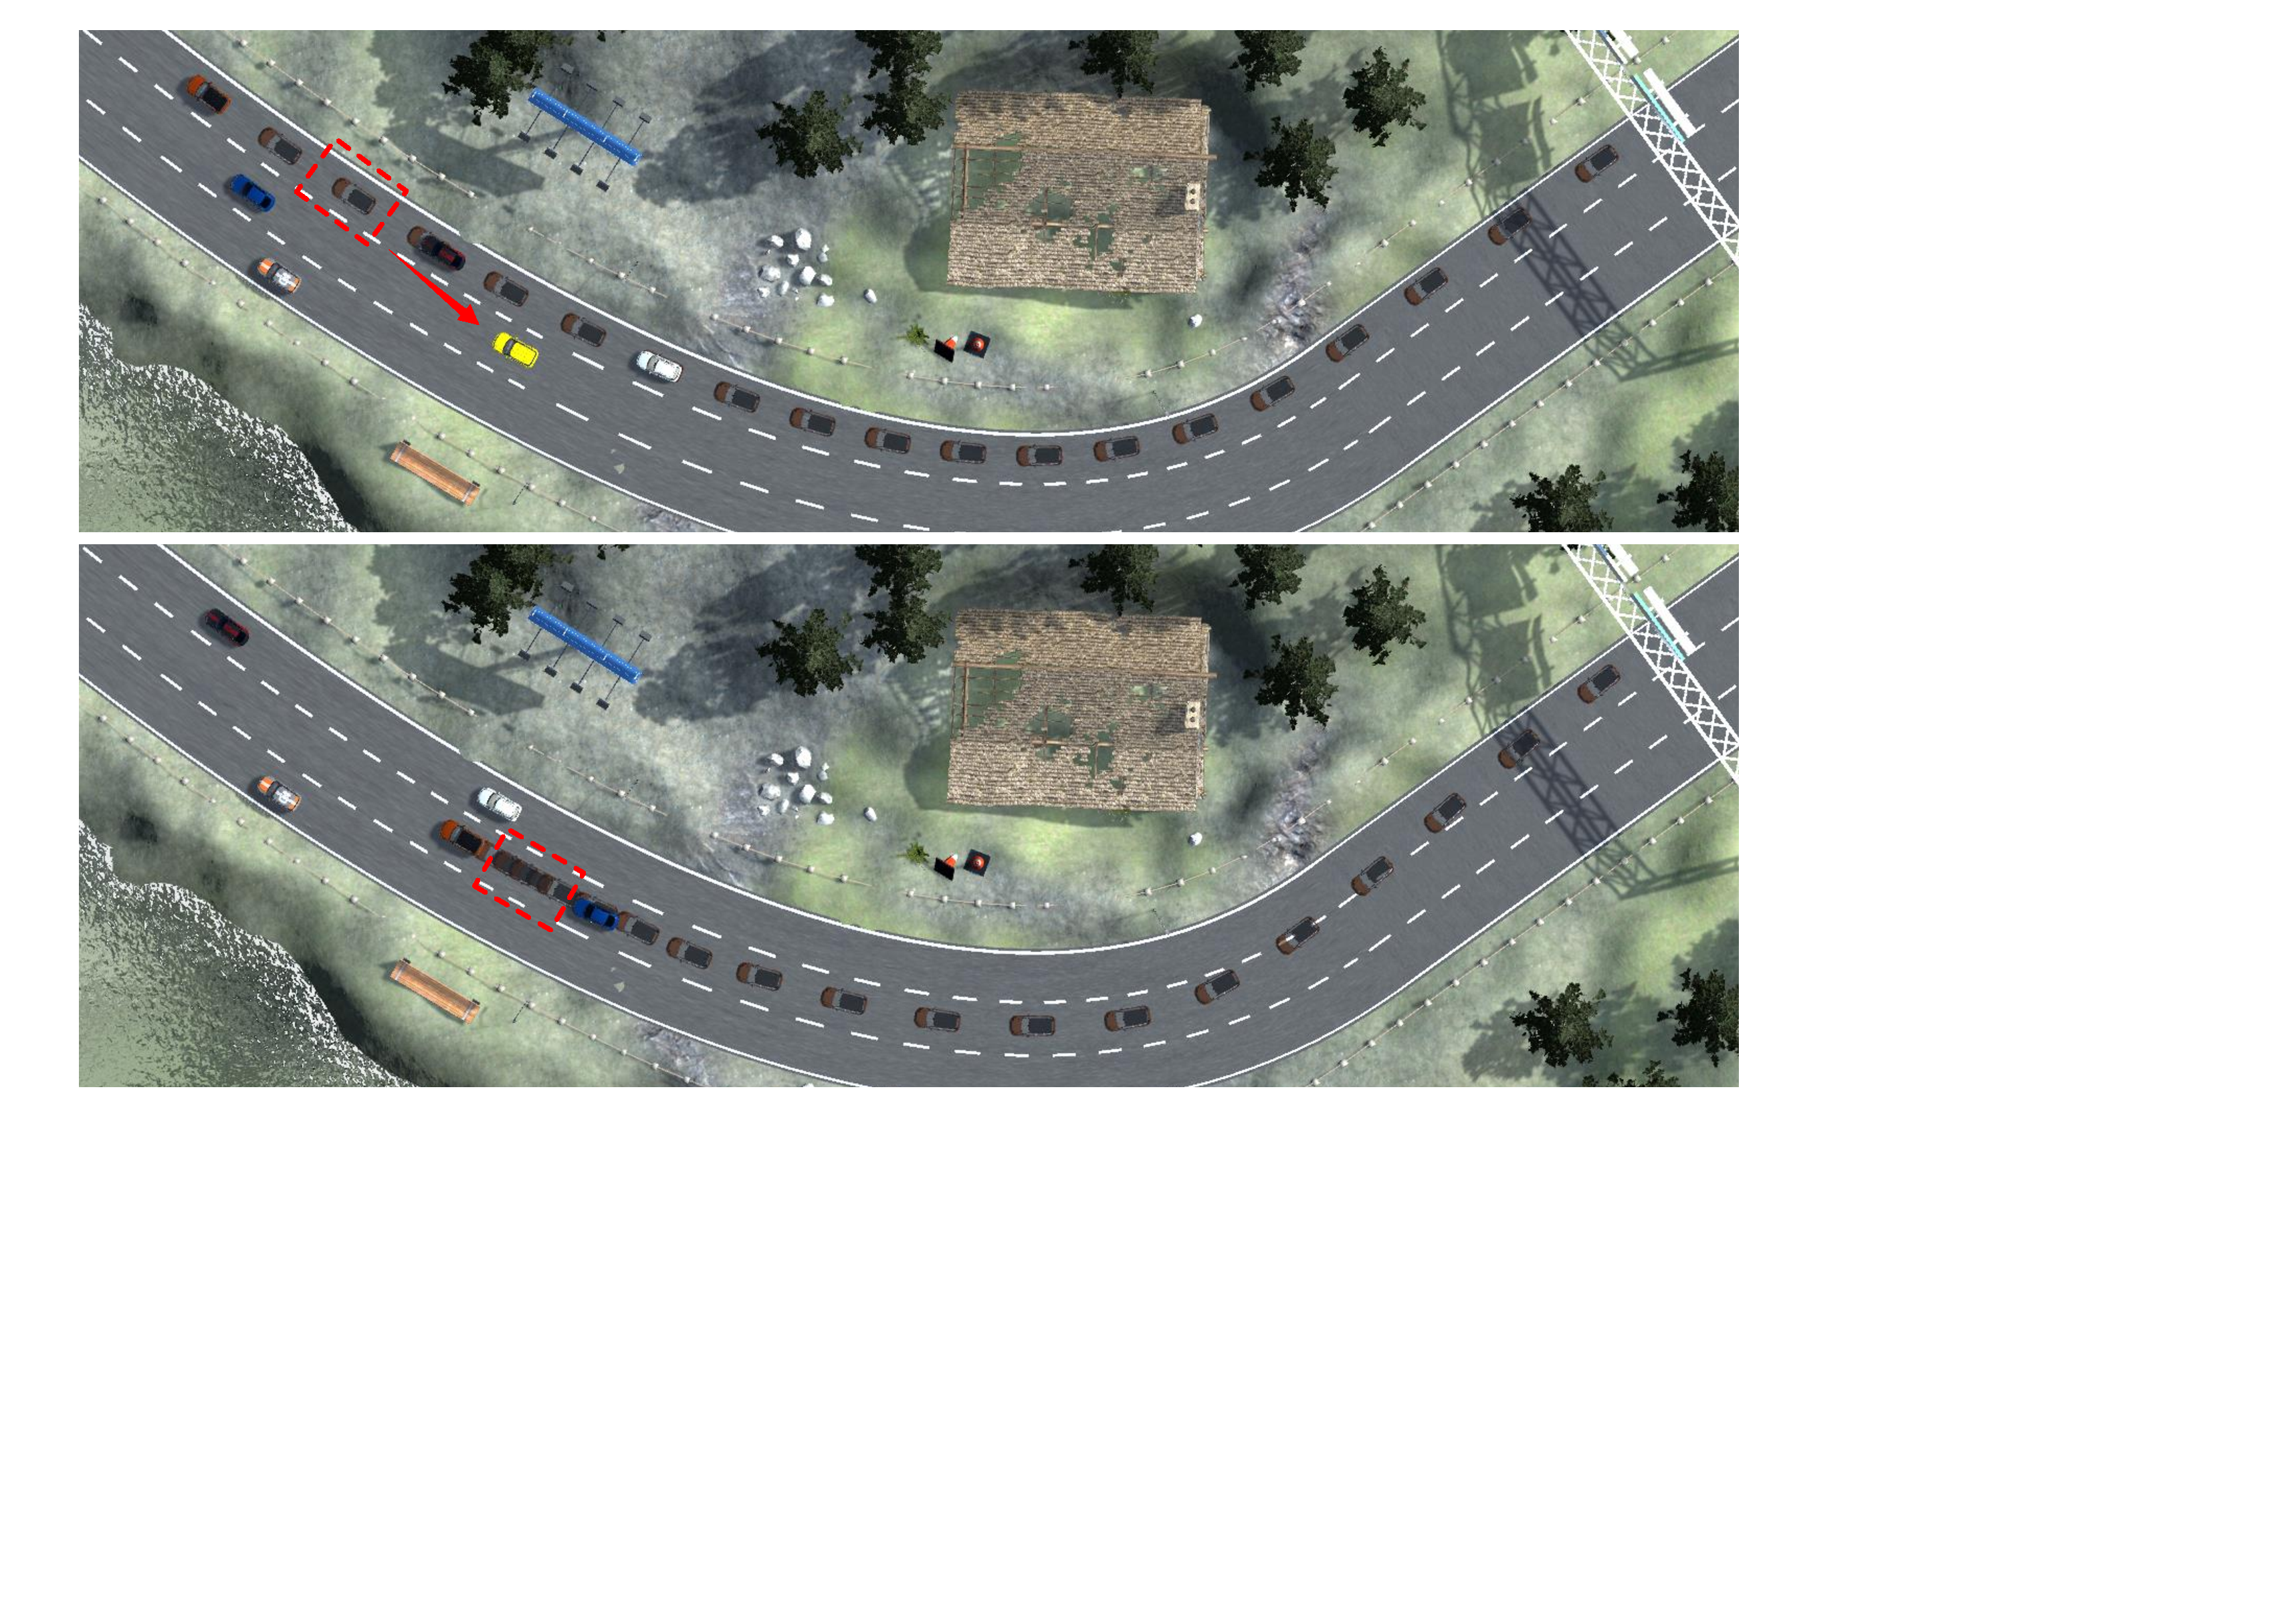
\includegraphics[width=0.87\textwidth]{figure/keyframe/case_bend_new_v2.pdf}
%\caption[弯道上使用关键帧控制车辆的交通仿真示意图]{
%(a) 原始轨迹。(b) 使用关键帧控制后的轨迹。目标车辆原本沿着最右侧的道路行驶,我们设置了一个关键帧在中间的车道上,表示我们希望目标车辆能够在红色虚线框出的时刻下到达该关键帧指定的位置。}
\caption[弯道超车关键帧控制编辑案例]{
弯道关键帧控制编辑案例
}
\label{fig:keyframe_teaser}
\end{figure}

第二个案例在包含人行横道的直道场景中生成,如图~\ref{fig:keyframe_caseredlight}所示。被编辑车辆原本在中间车道行驶,因红灯亮起停在了人行横道前,等待稍后依次通过。我们在最左侧车道设置了一个关键帧,令该车变道超车后快速通过人行横道而不要停留。最终,我们规划了一条穿过该位置点的新参考路径,车辆跟随该参考路径变道到一条未被前车阻塞的道路然后加速通过了人行横道。

\begin{figure}[!tbh]
\centering
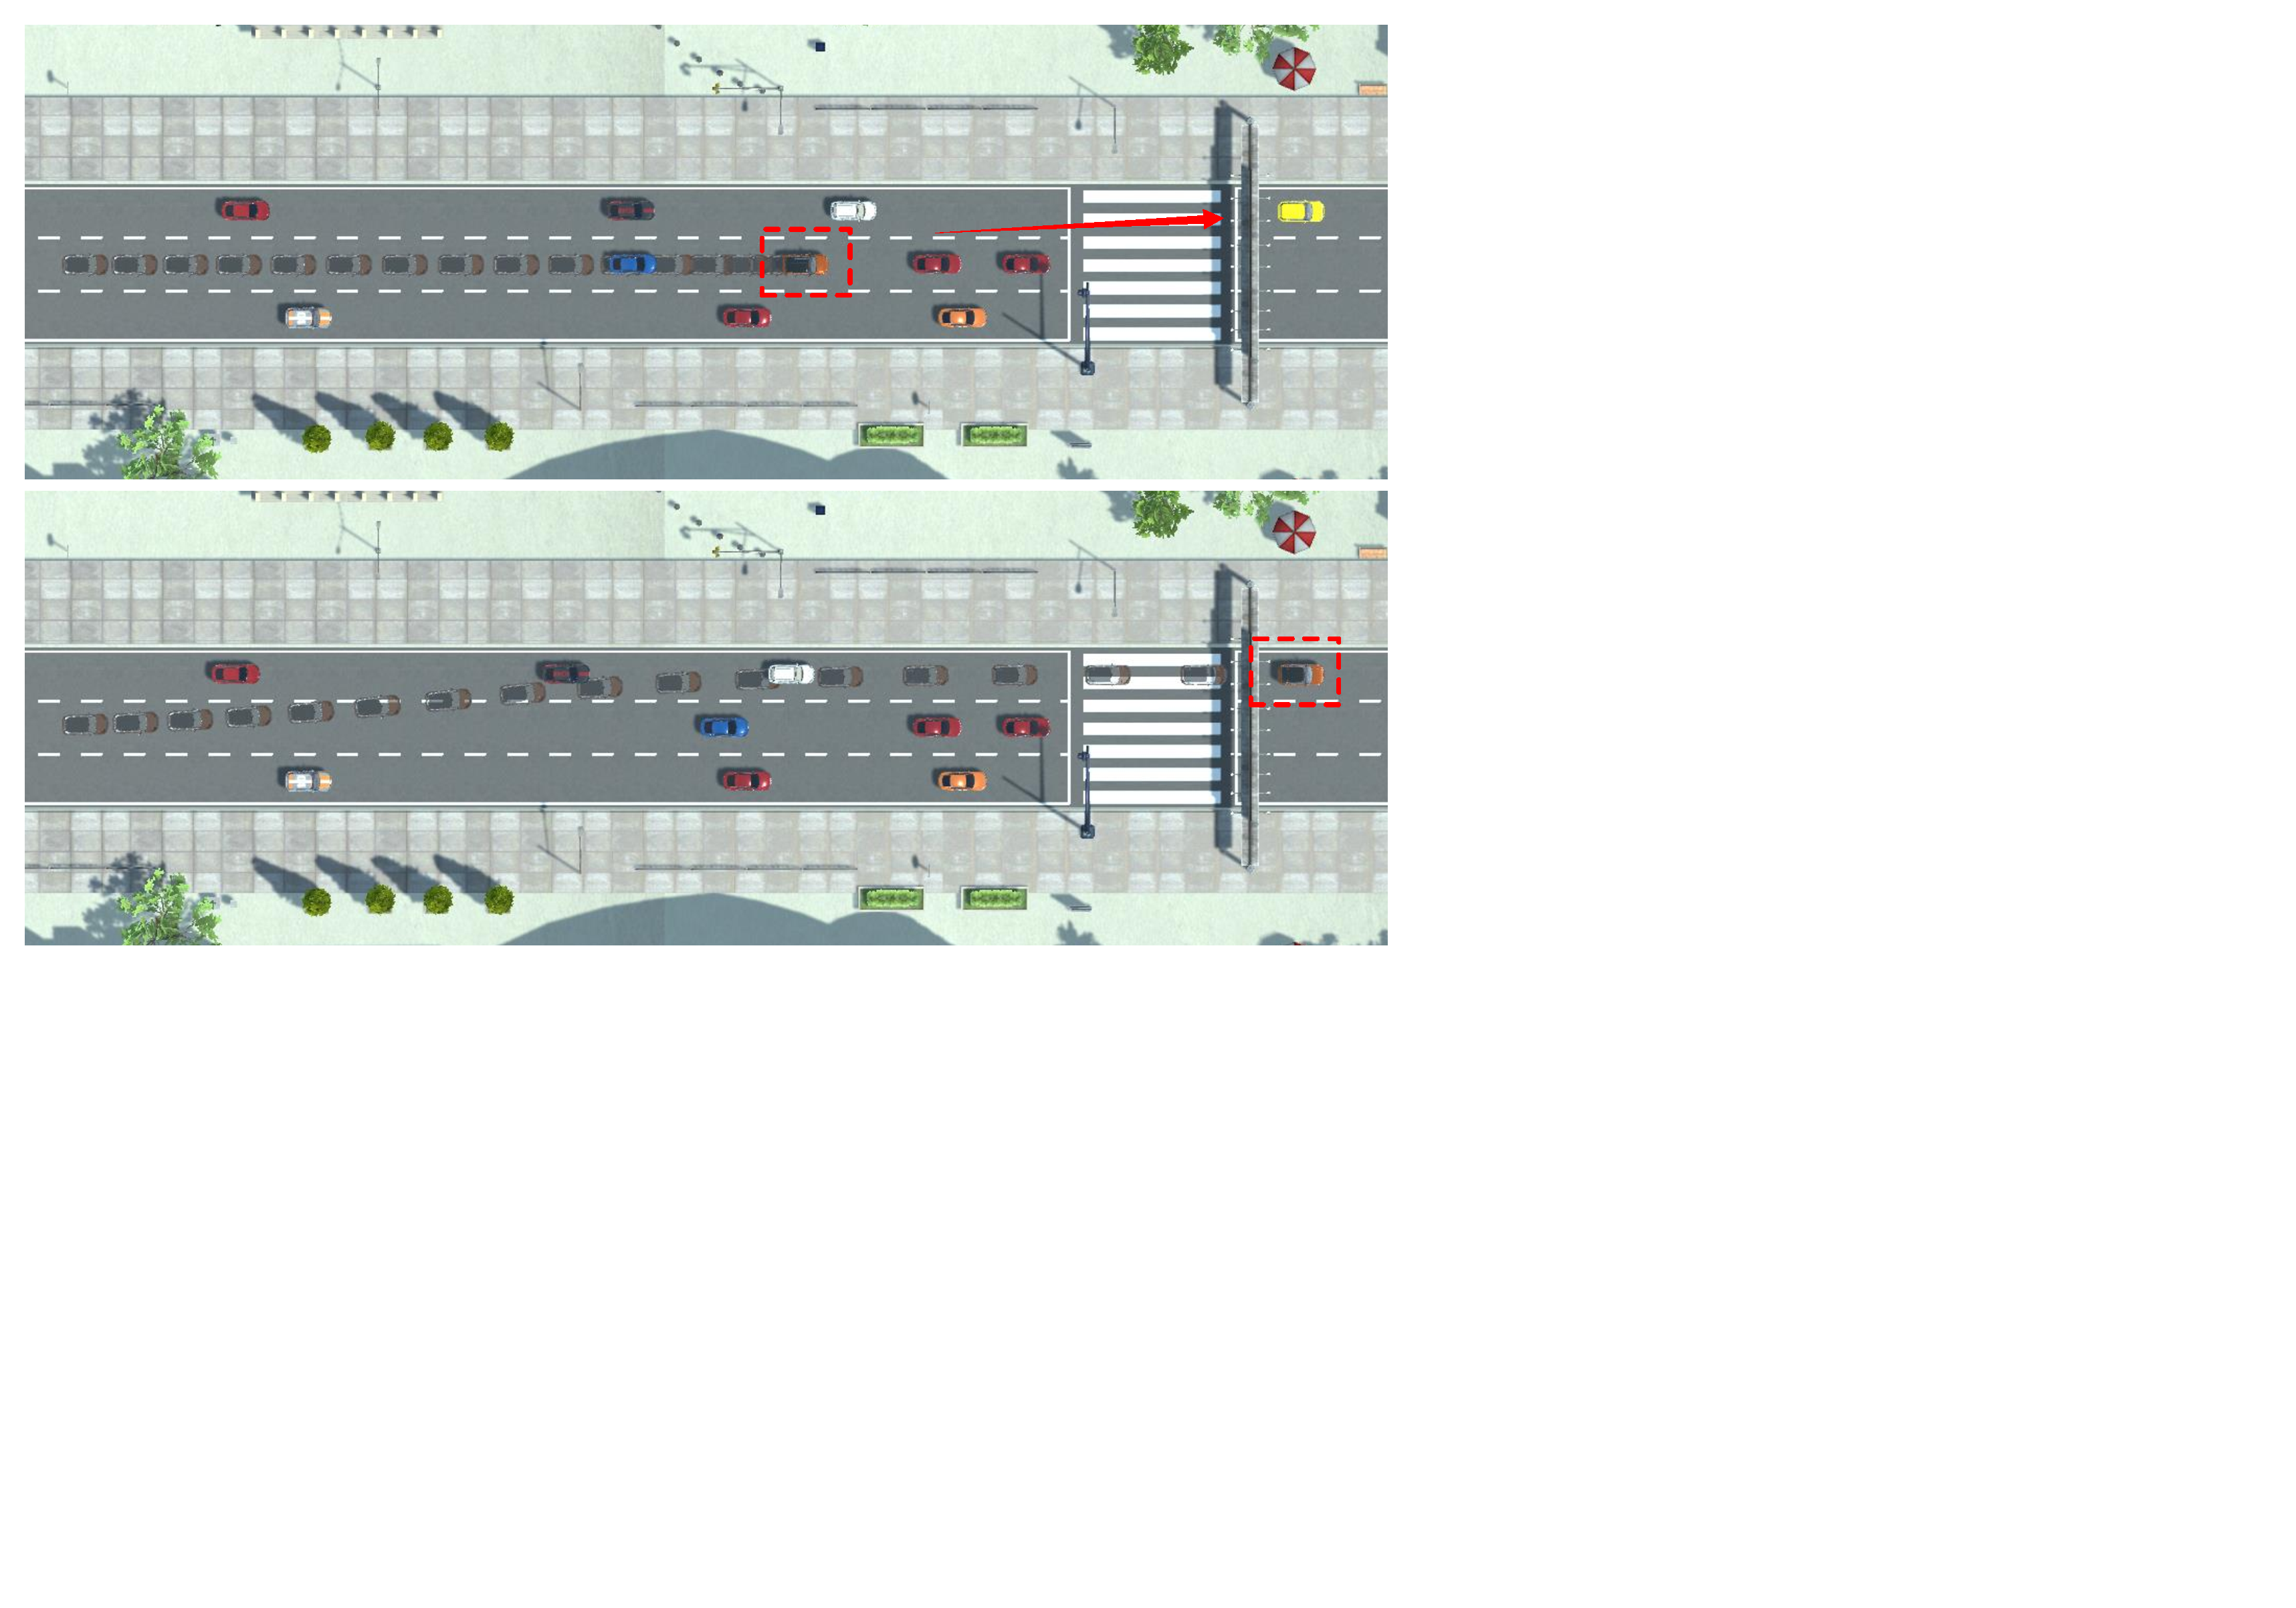
\includegraphics[width=0.82\columnwidth]{figure/keyframe/case_redlight_new_v2.pdf}
%\caption[人行横道闯红灯关键帧控制案例]{人行横道前闯红灯的原始轨迹(上)和关键帧控制轨迹(下)。}
\caption[人行横道闯红灯关键帧控制案例]{
人行横道闯红灯关键帧控制案例
}
\label{fig:keyframe_caseredlight}
\end{figure}

第三个案例在包含十字路口的场景生成,如图~\ref{fig:keyframe_caseintersection}所示。被编辑车辆原本行驶在左侧车道并计划右转弯,在通过路口时并未等待右侧车道的直行车辆先行。我们在通过路口前设置了一个关键帧,令该车在转向前进行等待。在这个案例中,我们无需生成新的参考路径,被编辑车辆只需要沿着原始参考路径就能满足关键帧的约束。最终,被编辑车辆在通过路口前提前减速直至停止,让右侧车道上的直行来车先行。

\begin{figure}[!tbh]
\centering
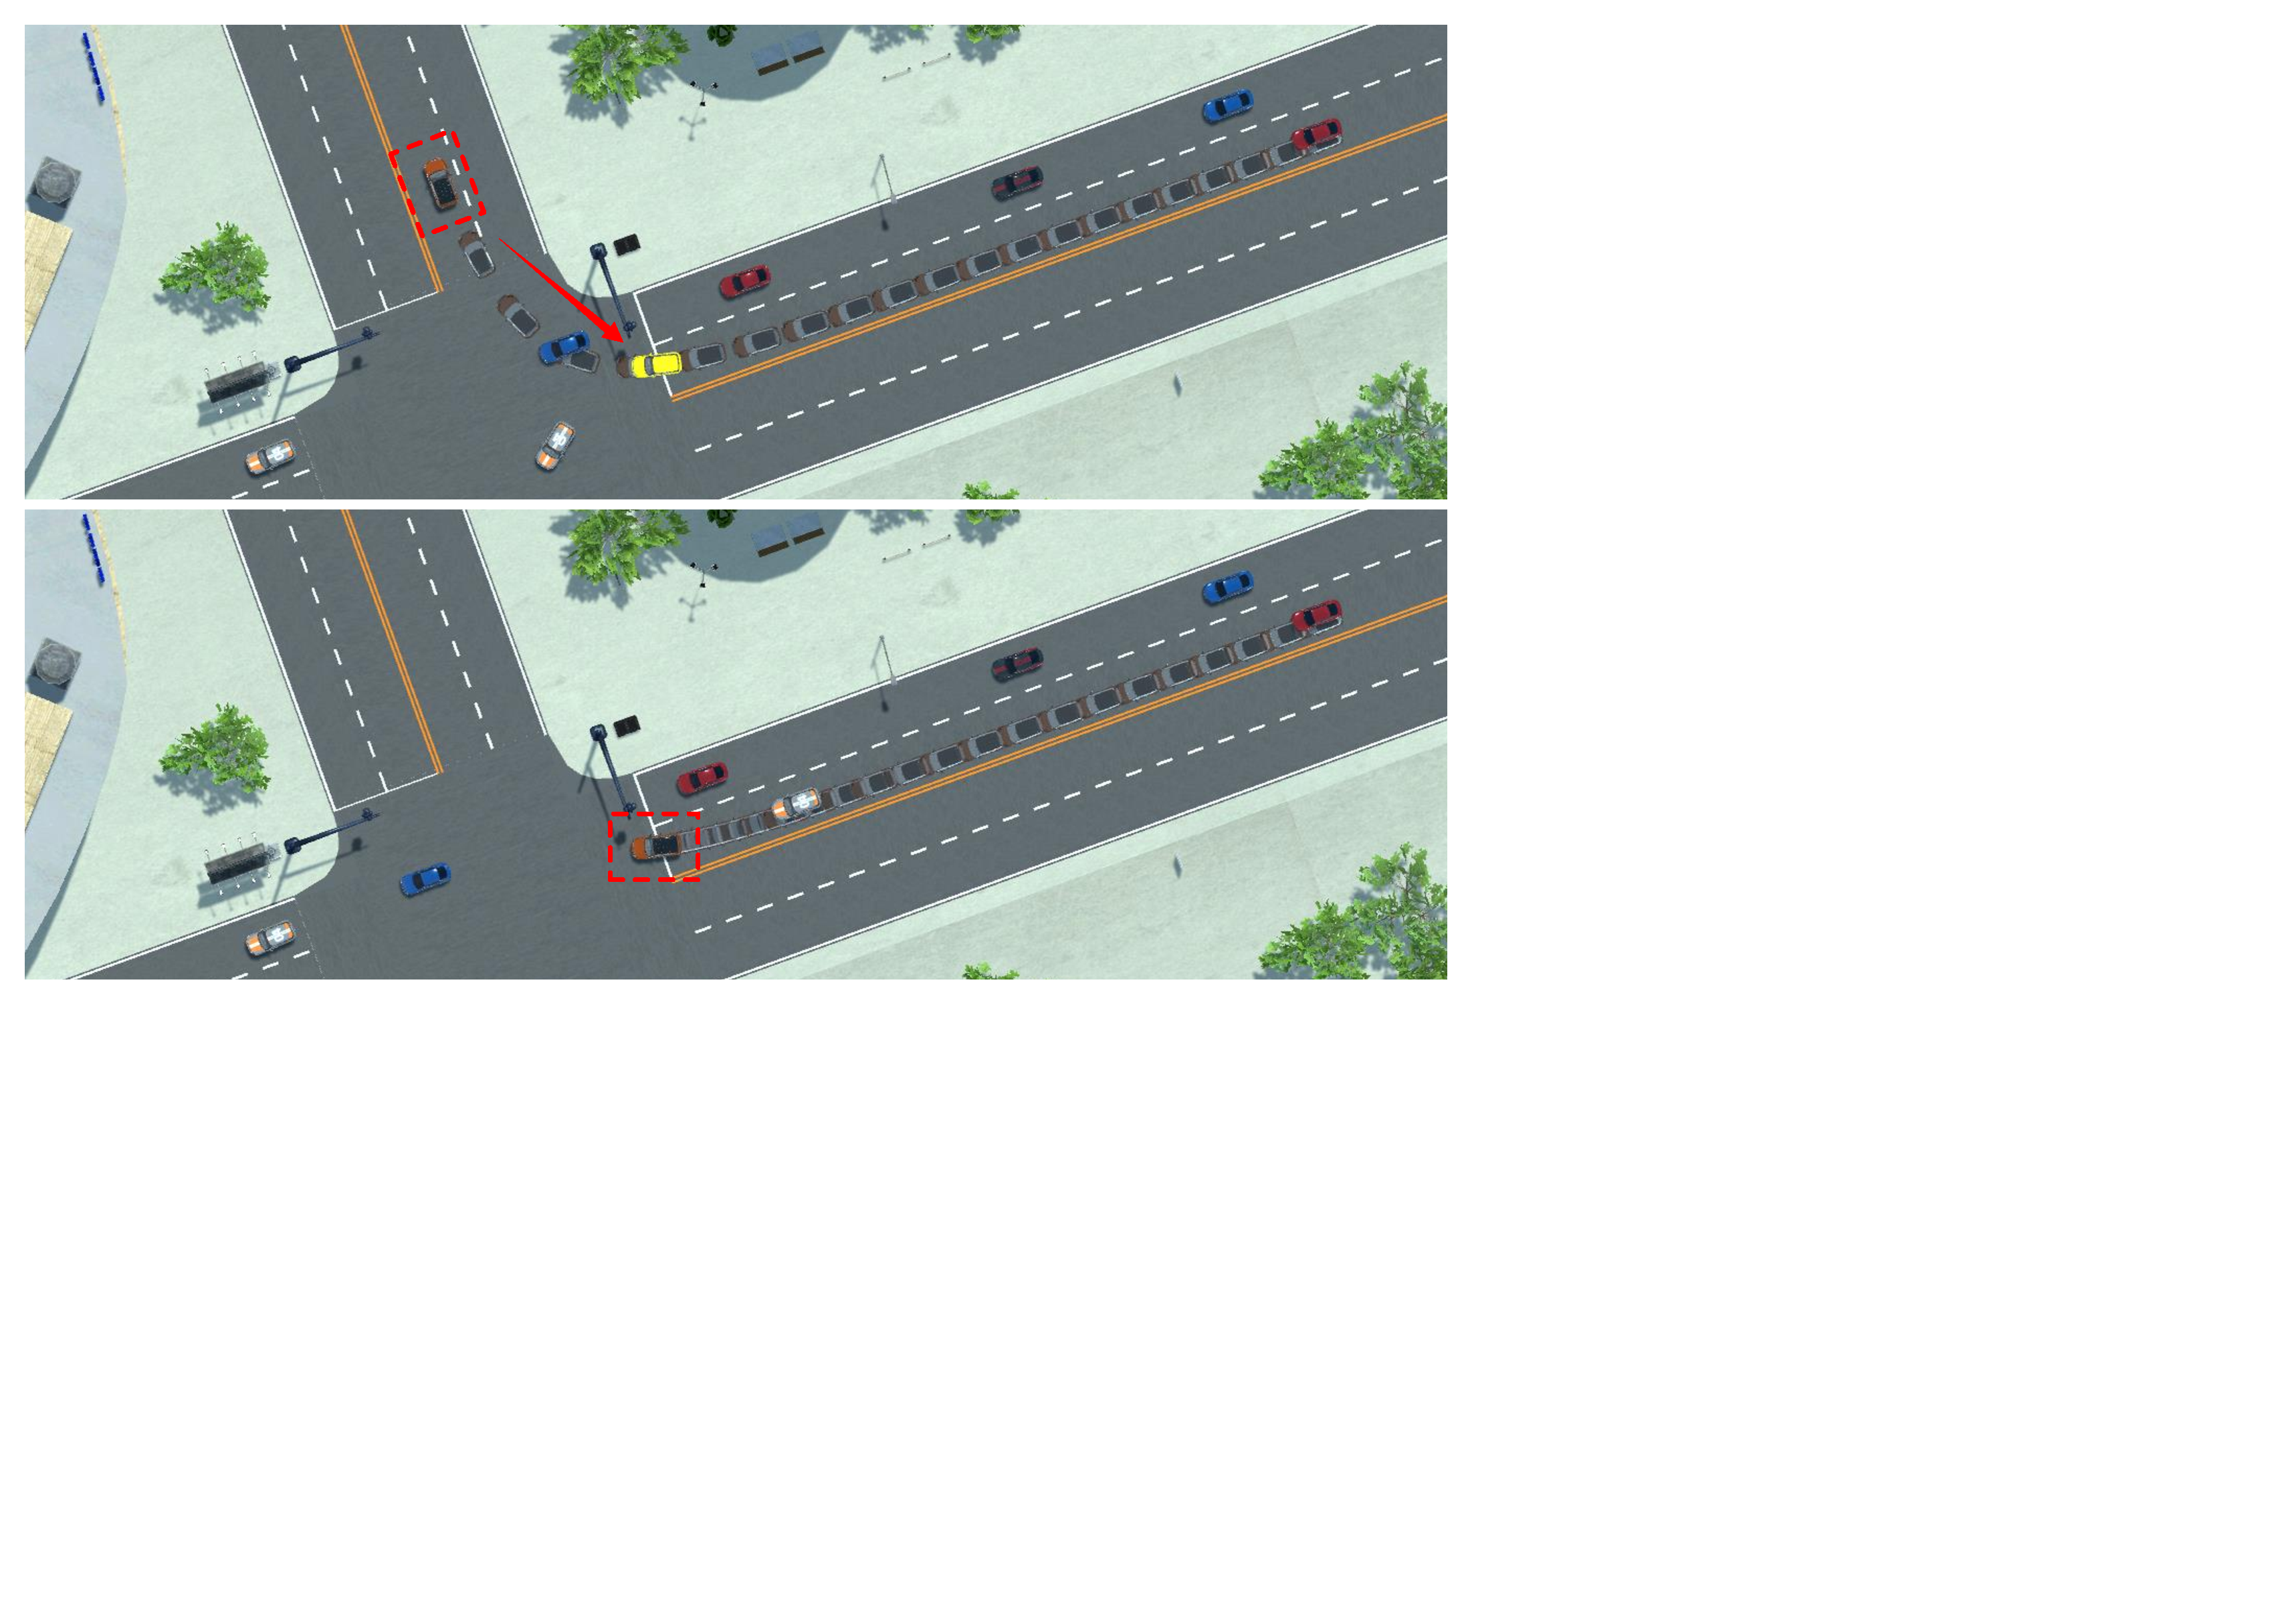
\includegraphics[width=0.82\columnwidth]{figure/keyframe/case_intersection_new_v2.pdf}
%\caption[十字路口避让来车关键帧控制案例]{在转弯通过十字口前避让后方来车的原始轨迹(上)和关键帧控制轨迹(下)。}
\caption[十字路口避让来车关键帧控制案例]{
十字路口避让来车关键帧控制案例
}
\label{fig:keyframe_caseintersection}
\end{figure}



\subsection{性能分析与对比}
\label{section:keyframe_performance}


为了验证我们提出的由粗到细优化求解关键帧的性能,我们设计了一系列实验,包含了不同的离散化时间步长或不同的伴随法初始化设置。后续实验均基于一个相同的关键帧生成,该关键帧控制车辆沿着其参考路径在10秒内前进100米,伴随法的梯度下降最大迭代次数为100次。

我们首先使用不同的离散化时间步长离散状态-时间空间以搜索粗粒度轨迹,取$\Delta{\Tilde{t}}$=0.5秒,0.25秒和0.1秒,表~\ref{tab:keyframe_sttperformance}中展示了对应搜索所需要的时间,其中$\Delta{\Tilde{t}}$=0.5秒为原先交通重建工作~\cite{sewall2010virtualized}中使用的设置。当$\Delta{\Tilde{t}}$逐渐变小,状态-时间空间离散化越精细,则状态-时间搜索得到的轨迹会越精细,但是搜索同样也会急速增长。根据表~\ref{tab:keyframe_sttperformance}所示,当$\Delta{\Tilde{t}}$=0.25秒时,搜索路径的总耗时为36.924秒;而当$\Delta{\Tilde{t}}$=0.1秒时,由于超出了内存的限制,已经无法统计对应的搜索耗时。因此如之前所述,在状态-时间空间中,想要通过减小离散化时间步长来提高基于关键帧搜索的轨迹结果是不切实际的。

\begin{table}[!tbh]
% first table
\begin{minipage}[!tbh]{\columnwidth}
%\setlength{\abovecaptionskip}{-0.05cm} 
\setlength{\belowcaptionskip}{0.4cm}
\renewcommand{\arraystretch}{1.7}
\centering
%\caption[不同离散化时间步长的状态-时间搜索耗时统计]{不同离散化时间步长(秒)下,状态-时间的搜索耗时(秒)。当离散化时间步长为0.1秒时,由于超出内存限制已经无法统计对应的搜索耗时。}
\caption[不同离散化时间步长的状态-时间搜索耗时统计]{
不同离散化时间步长的状态-时间搜索耗时统计(单位:秒)
}
\setlength{\tabcolsep}{3.3mm}
{
    \begin{tabular}{|c|c|}
    \hline
    \textbf{离散时间步长} $\Delta{\Tilde{t}}$ & \textbf{状态-时间搜索耗时} \\ \hline
    0.5                     & 0.173                  \\ \hline
    0.25                    & 36.924                 \\ \hline
    0.1                     & $-$                      \\ \hline
    \end{tabular}
}
%\caption{The state-time search time (s) over different discretization timesteps (s). Due to memory limitation, it is hardly to obtain the state-time search time when discretization timestep is 0.1s.}
\label{tab:keyframe_sttperformance}
\vspace{2mm}
\end{minipage}

% second table
\begin{minipage}[!tbh]{\columnwidth}
%\setlength{\abovecaptionskip}{-0.05cm} 
\setlength{\belowcaptionskip}{0.4cm}
\renewcommand{\arraystretch}{1.7}
\centering
%\caption[不同仿真时间步长的伴随法求解耗时统计]{不同仿真步长(秒)下,求解伴随法的耗时(秒)。}
\caption[不同仿真时间步长的伴随法求解耗时统计]{
不同仿真时间步长的伴随法求解耗时统计(单位:秒)
}
\setlength{\tabcolsep}{4.7mm}
{
    \begin{tabular}{|c|c|}
    \hline
    \textbf{仿真时间步长} $\Delta{t}$ & \textbf{伴随法求解耗时} \\ \hline
    0.5                 & 0.002                           \\ \hline
    0.1                 & 0.004                           \\ \hline
    0.05                & 0.011                           \\ \hline
    0.01                & 0.185                           \\ \hline
    0.005               & 0.699                           \\ \hline
    \end{tabular}
}
%\caption{The adjoint-based optimization time (s) over different traffic simulation timesteps (s) for a certain trajectory.}
\label{tab:keyframe_adjperofmance}
\end{minipage}
\end{table}


然后我们基于不同的仿真时间步长来求解伴随法,取$\Delta{t}$=0.5秒,0.1秒,0.05秒,0.01秒和0.005秒,表~\ref{tab:keyframe_adjperofmance}中展示了对应优化过程所需要的时间。显然,在给定梯度下降迭代次数的情况下,伴随法的求解时间主要依赖于待优化轨迹的长度,即轨迹中包含的帧数。因此当$\Delta{t}$逐渐变小,优化过程会变得越发耗时。在代码实现中,我们在生成轨迹的质量和优化过程的耗时之间取舍后,选取$\Delta{\Tilde{t}}$=0.5秒和$\Delta{t}$=0.01秒。因此对于测试实验的设置而言,我们的方法在梯度下降迭代100次时生成一整条关键帧控制的轨迹只需要花费0.358秒。


我们对比了仅使用状态-时间搜索方法生成的轨迹结果与使用我们提出的由粗到细求解约束生成的轨迹结果,图~\ref{fig:keyframe_comparison}(a)中展示的是两条轨迹中沿着路径方向的速度分量。仅用状态-时间搜索方法生成的轨迹速度存在瞬时突变,这是由于轨迹是在大尺度离散化的空间中搜索生成的,且车辆仅能从确定元素的集合中选取加速度的值。相比之下,我们提出的由粗到细求解约束生成的轨迹速度变化更加的连续、平滑。

\begin{figure}[!tbh]
\centering
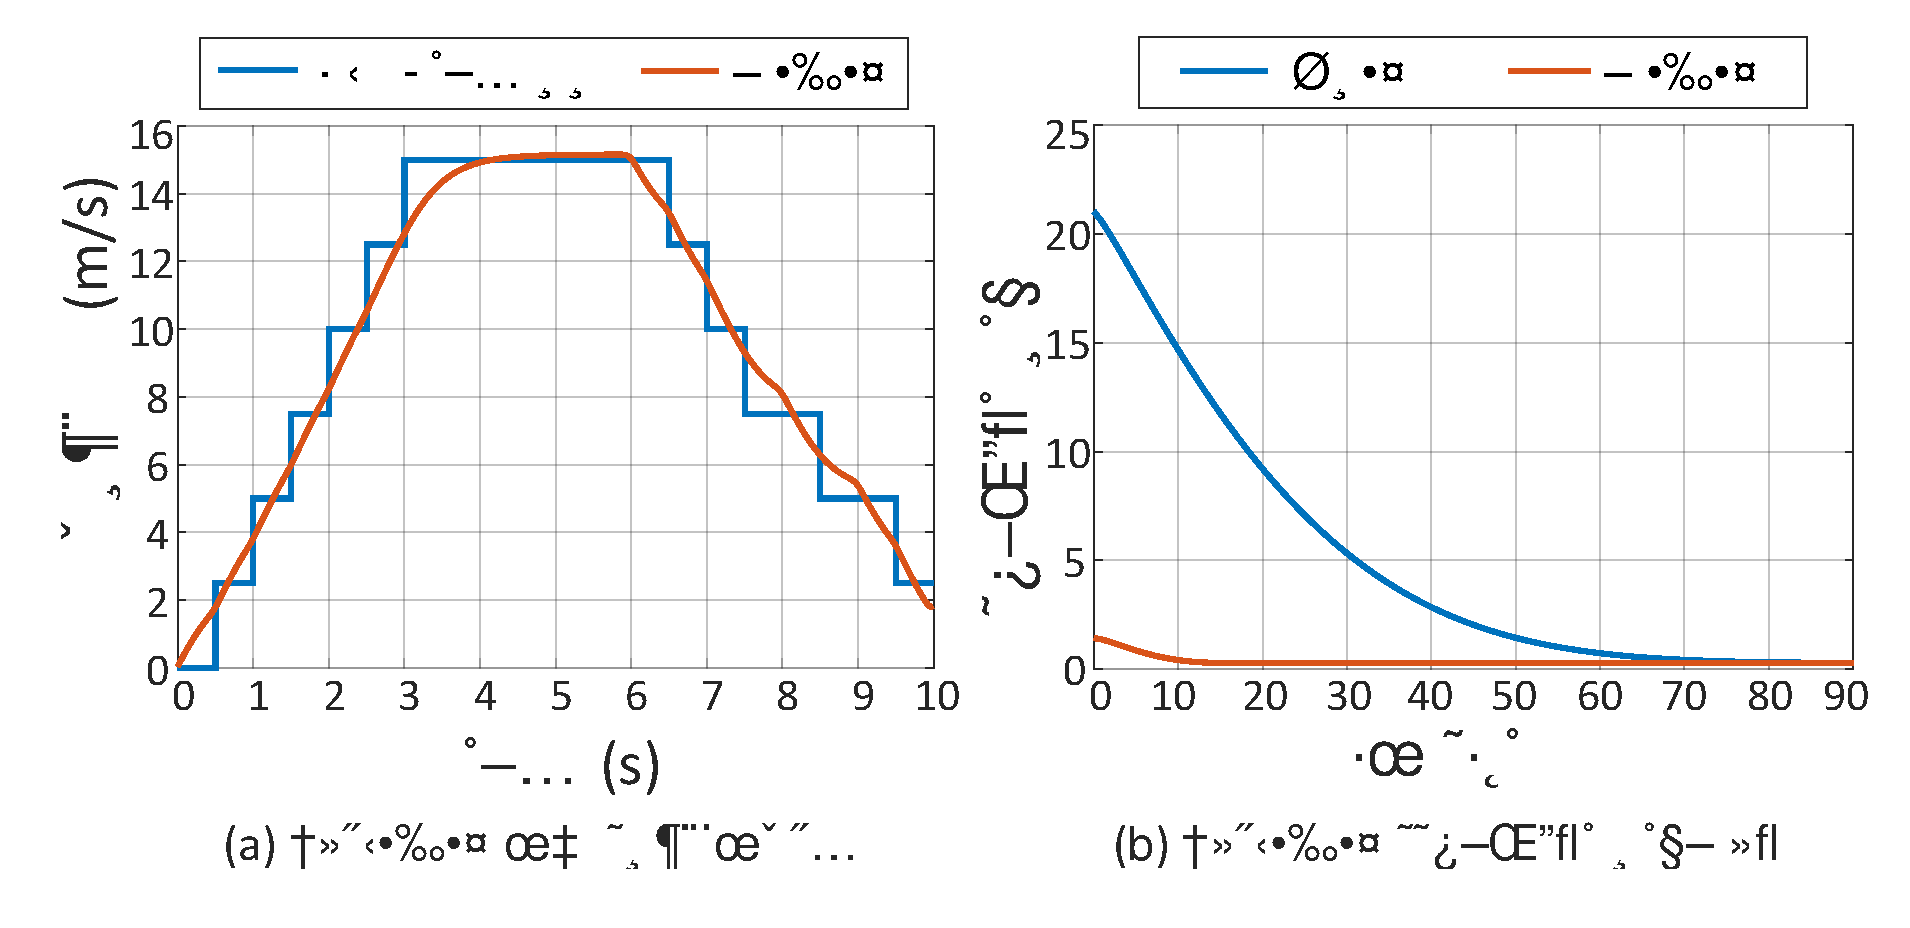
\includegraphics[width=0.85\columnwidth]{figure/keyframe/comparisons_v3_cn.pdf}
%\caption[对比实验结果示意图]{(a) 仅使用状态-时间搜索生成的轨迹与使用我们提出的由粗到细求解约束生成的轨迹的沿着路径方向的速度。(b) 梯度下降过程中每一次迭代目标函数当前的损失值,其中伴随法表示将待优化控制预期速度初始化为规定时间内完成所需位移的平均速度。}
\caption[对比实验结果]{
对比实验结果
}
\label{fig:keyframe_comparison}
\end{figure}

我们又对比了使用不同的初始化策略时,梯度下降的过程中每一次迭代目标函数当前的损失值,图~\ref{fig:keyframe_comparison}(b)中展示的分别是使用按时完成路径轨迹的平均速度初始化的结果,和使用我们在状态-时间中搜索出的粗粒度轨迹初始化的结果。在使用平均速度作为初始值时,伴随法在约70次迭代时能够达到收敛,相比之下使用粗粒度的轨迹作为初始值时,伴随法则能在15次迭代时就达到收敛,且初始时的目标函数损失就已经非常小。因此在实际代码实现过程中,我们可以根据伴随法的梯度收敛情况适当提前停止优化迭代,进一步减少计算时间。


最后,表~\ref{tab:keyframe_cmpmethods}中总结展示了本方法和之前相关研究在关键方面的对比。本方法包括了之前方法的所有优点,如能生成平滑的运动,允许在复杂的场景中进行仿真,且在仿真过程中能够交互式控制和编辑车辆。此外,由于我们的交通仿真基于社会力模型,因此我们可以通过求解时-空关键帧的约束来控制车辆运动,使得轨迹编辑的方式更灵活,生成预期轨迹和场景数据的过程更简洁。



\begin{table}[!tbh]
%\setlength{\abovecaptionskip}{-0.05cm} 
\setlength{\belowcaptionskip}{0.4cm}
\centering
\normalsize
\renewcommand\arraystretch{1.5}
%\caption[与之前方法的对比总结]{与之前方法的对比总结。我们考虑如下几个方面或评判标准 (a) 交通仿真模型,(b) 是否能生成平滑的运动,(c) 是否允许在复杂的场景中仿真,(d) 是否允许交互式控制和编辑仿真中的车辆,(e) 是否允许使用时-空关键帧来约束车辆行为。}
\caption[与之前方法的对比总结]{
与之前方法的对比总结
}
\begin{tabular}{|c|c|c|c|c|c|}
%Method & Simulation Model & Complex Scenarios & Interactively Editing & Spatial-Temporal Keyframes \\
\hline
\textbf{方法} & \textbf{仿真模型} & \textbf{运动平滑} & \textbf{复杂场景} & \textbf{交互式编辑} & \textbf{关键帧} \\ \hline
Sewall等人~\cite{sewall2010virtualized}    & 状态\-时间搜索 & \ding{55} & \ding{51} & \ding{55} &\ding{51} \\ \hline
Chao等人~\cite{chao2021calibrated}       & 社会力模型 & \ding{51} & \ding{55} & \ding{55} & \ding{55} \\ \hline
TraEDITS & 数据驱动 & \ding{51} & \ding{51}   & \ding{51}   & \ding{55} \\ \hline
Ours                            & 社会力模型 & \ding{51} & \ding{51}   & \ding{51}   & \ding{51}   \\ \hline
\end{tabular}
\label{tab:keyframe_cmpmethods}
\end{table}



\subsection{失败案例与修复}
\label{section:keyframe_failure}

为了展示本方法生成预期交通轨迹的能力,我们展示了部分编辑失败的案例,同时我们又使用本方法对这些失败案例进行迭代式的修复,人工指定更多的关键帧来完善不正确的交通行为。

第一个失败案例如图~\ref{fig:keyframe_failure1}(a)所示,被编辑车辆由于交通堵塞而没能在指定时间到达关键帧的位置。我们提供两个解决方法:第一个解决方案是赋予被编辑车辆另一个关键帧,使其从邻车道超车而越过受前车阻挡的位置,如图~\ref{fig:keyframe_failure1}(b)所示;第二个解决方案是为两辆前车分别赋予关键帧,使他们变道从而让出中间的车道给被编辑车辆加速行驶,如图~\ref{fig:keyframe_failure1}(c)所示。最终,上述两种解决方案均能使原本失败的关键帧控制变为成功。

第二个失败案例如图~\ref{fig:keyframe_failure2}(b)所示,被编辑车辆在进行U型掉头时保持了一个与实际不符的高速,在生活中司机在过急弯道时通常会降低速度以确保安全和舒适性。我们同样提供了两个解决方案:第一个解决方案是赋予被编辑车辆另一个关键帧,使其在掉头之前减速到达一个安全过弯速度,如图~\ref{fig:keyframe_failure2}(b)所示;第二个解决方案是赋予被编辑车辆另两个关键帧,一个使其在掉头之前制动,等待对向来车先行通过,另一个使其恢复原始的速度通过U型路段,从而避免激进或不文明的驾驶行为,如图~\ref{fig:keyframe_failure2}(c)所示。


\begin{figure}[!tbh]
%\setlength{\abovecaptionskip}{-0.1cm} 
%\setlength{\belowcaptionskip}{-0.45cm}
\centering
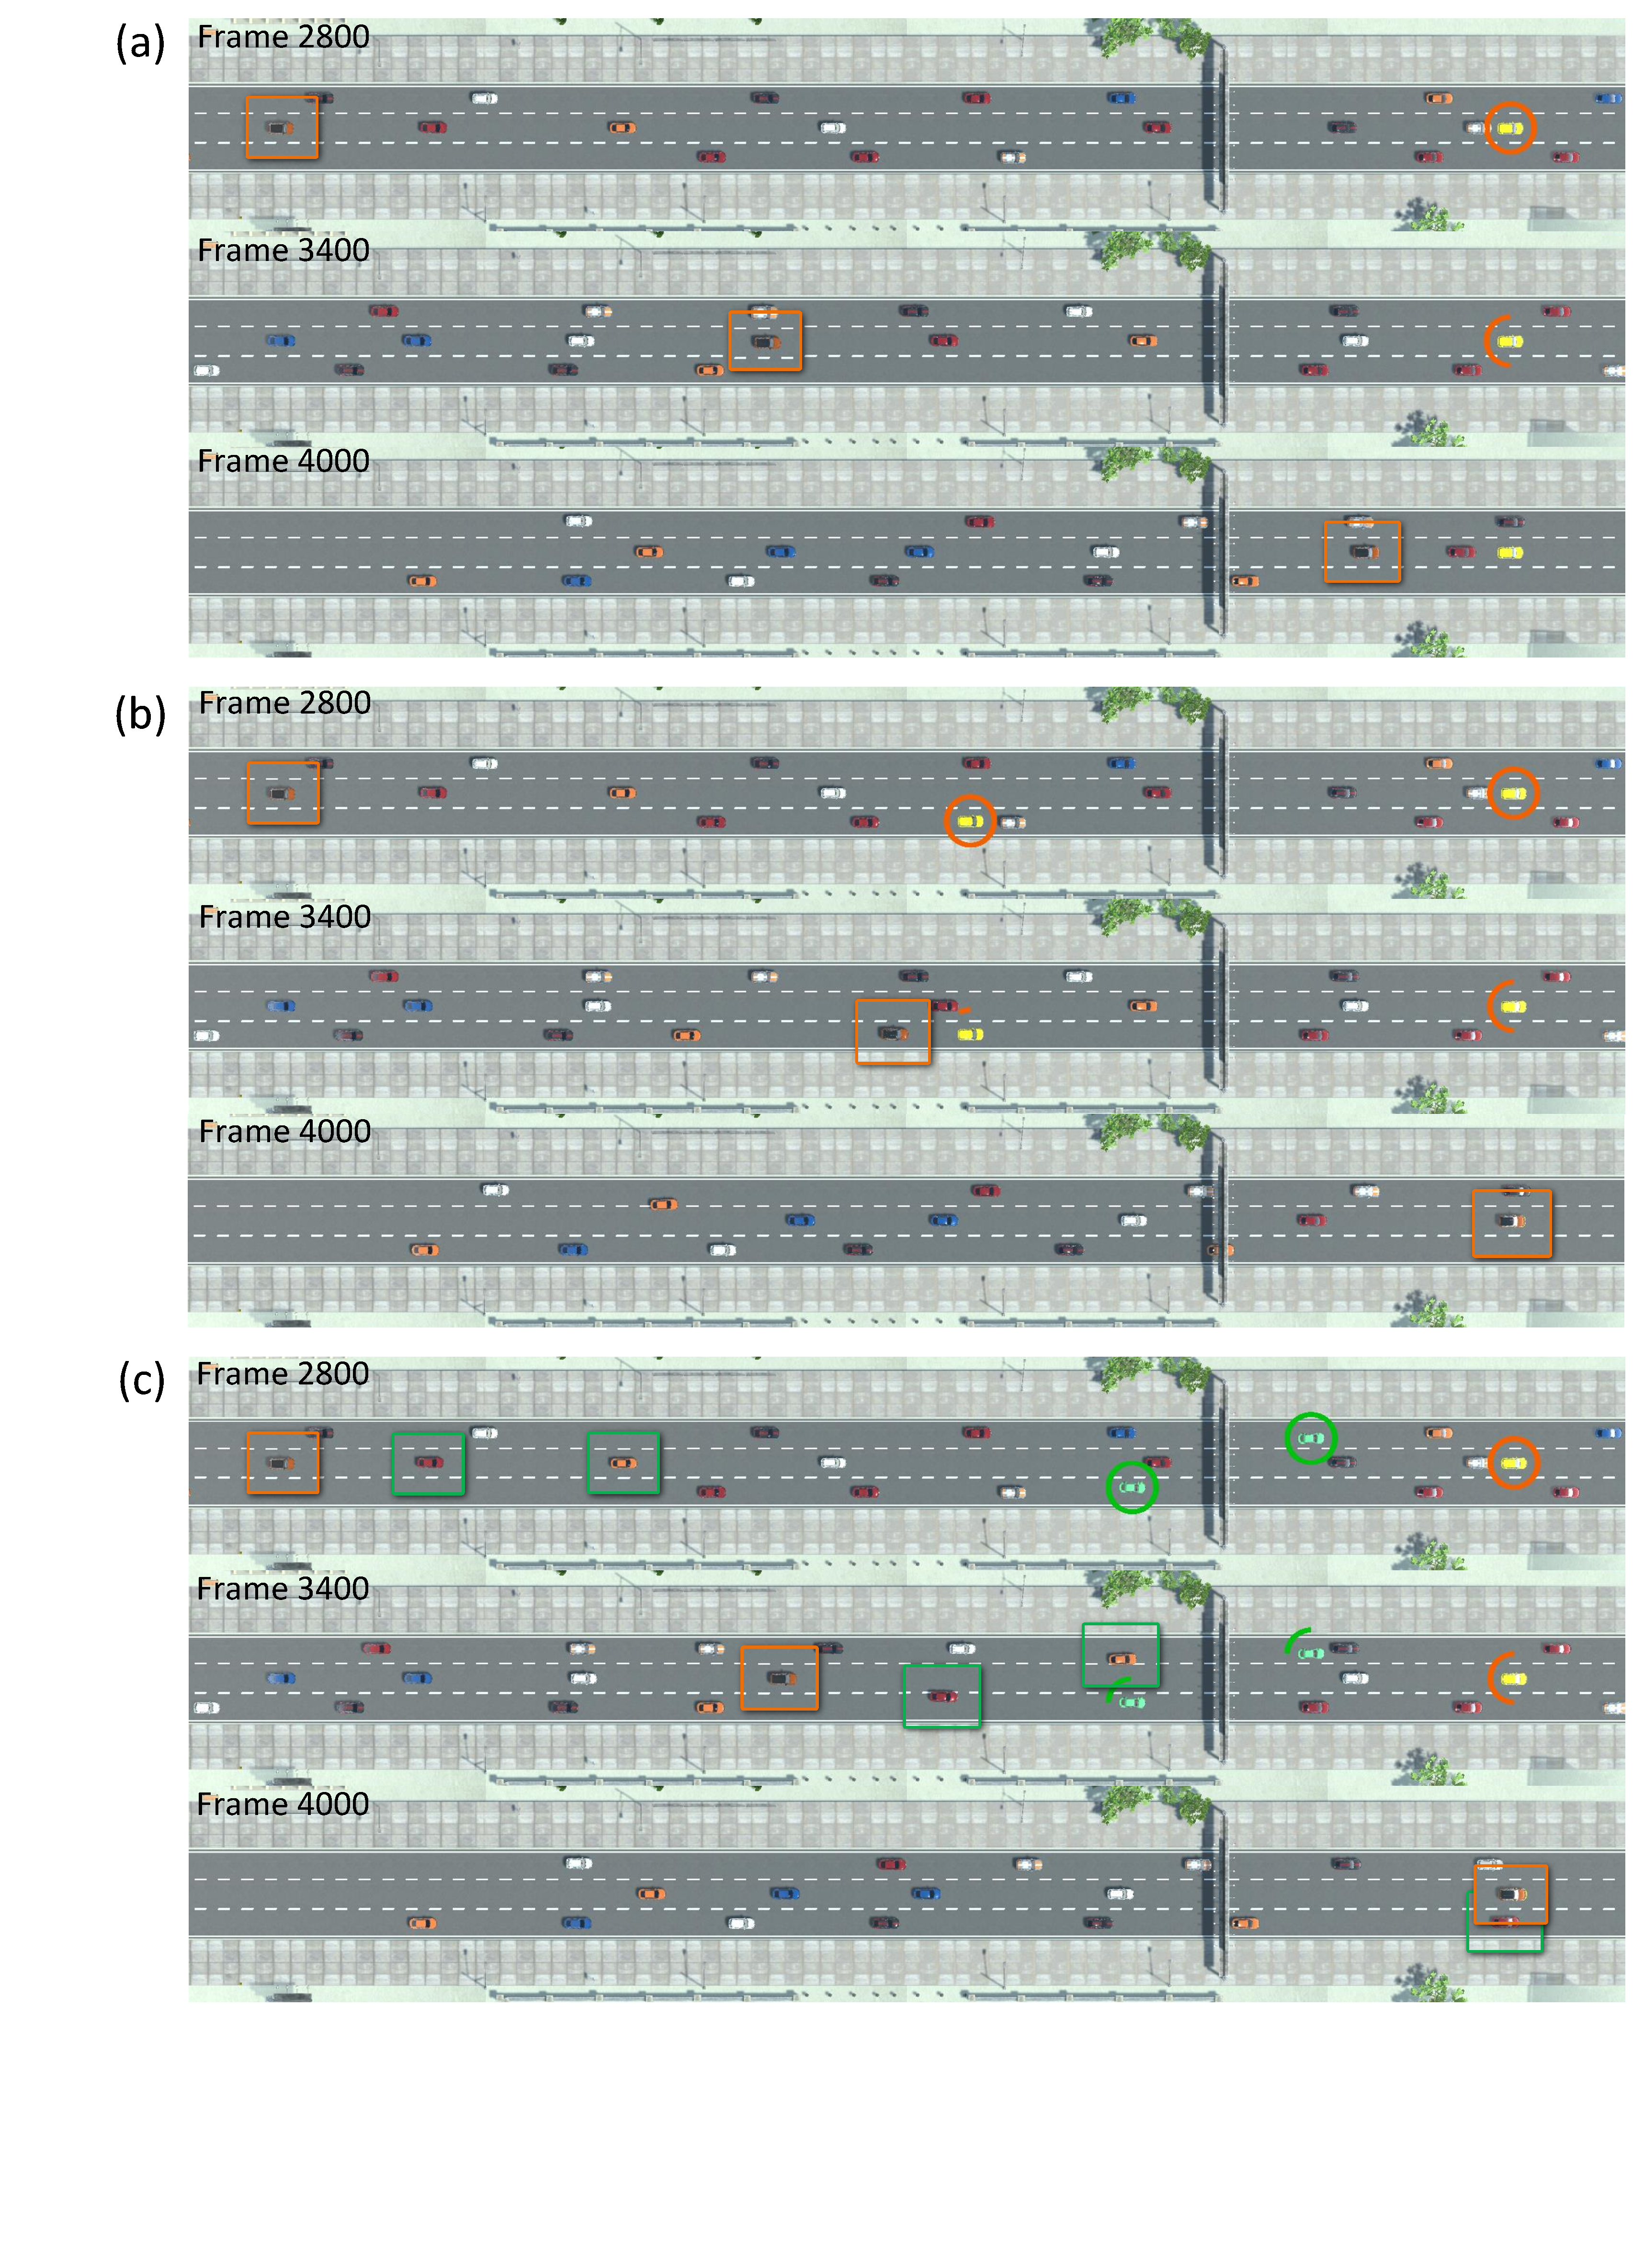
\includegraphics[width=0.91\textwidth]{figure/keyframe/failure_cases1_v3.pdf}
%\caption[因前车阻挡而失败的案例与修复结果]{第一个失败案例。(a) 被编辑车辆由于前车阻挡而没能在指定时间到达关键帧的位置。(b) 第一个解决办法是赋予其另一个关键帧,使其从邻车道超车而越过受前车阻挡的位置。(c) 第二个解决办法是为两辆前车分别赋予关键帧,使他们变道从而让出中间的车道。}
\caption[因前车阻挡而失败的案例与两种修复结果]{
因前车阻挡而失败的案例与两种修复结果
}
\label{fig:keyframe_failure1}
\end{figure}


\begin{figure}[!tbh]
%\setlength{\abovecaptionskip}{-0.1cm} 
%\setlength{\belowcaptionskip}{-0.45cm}
\centering
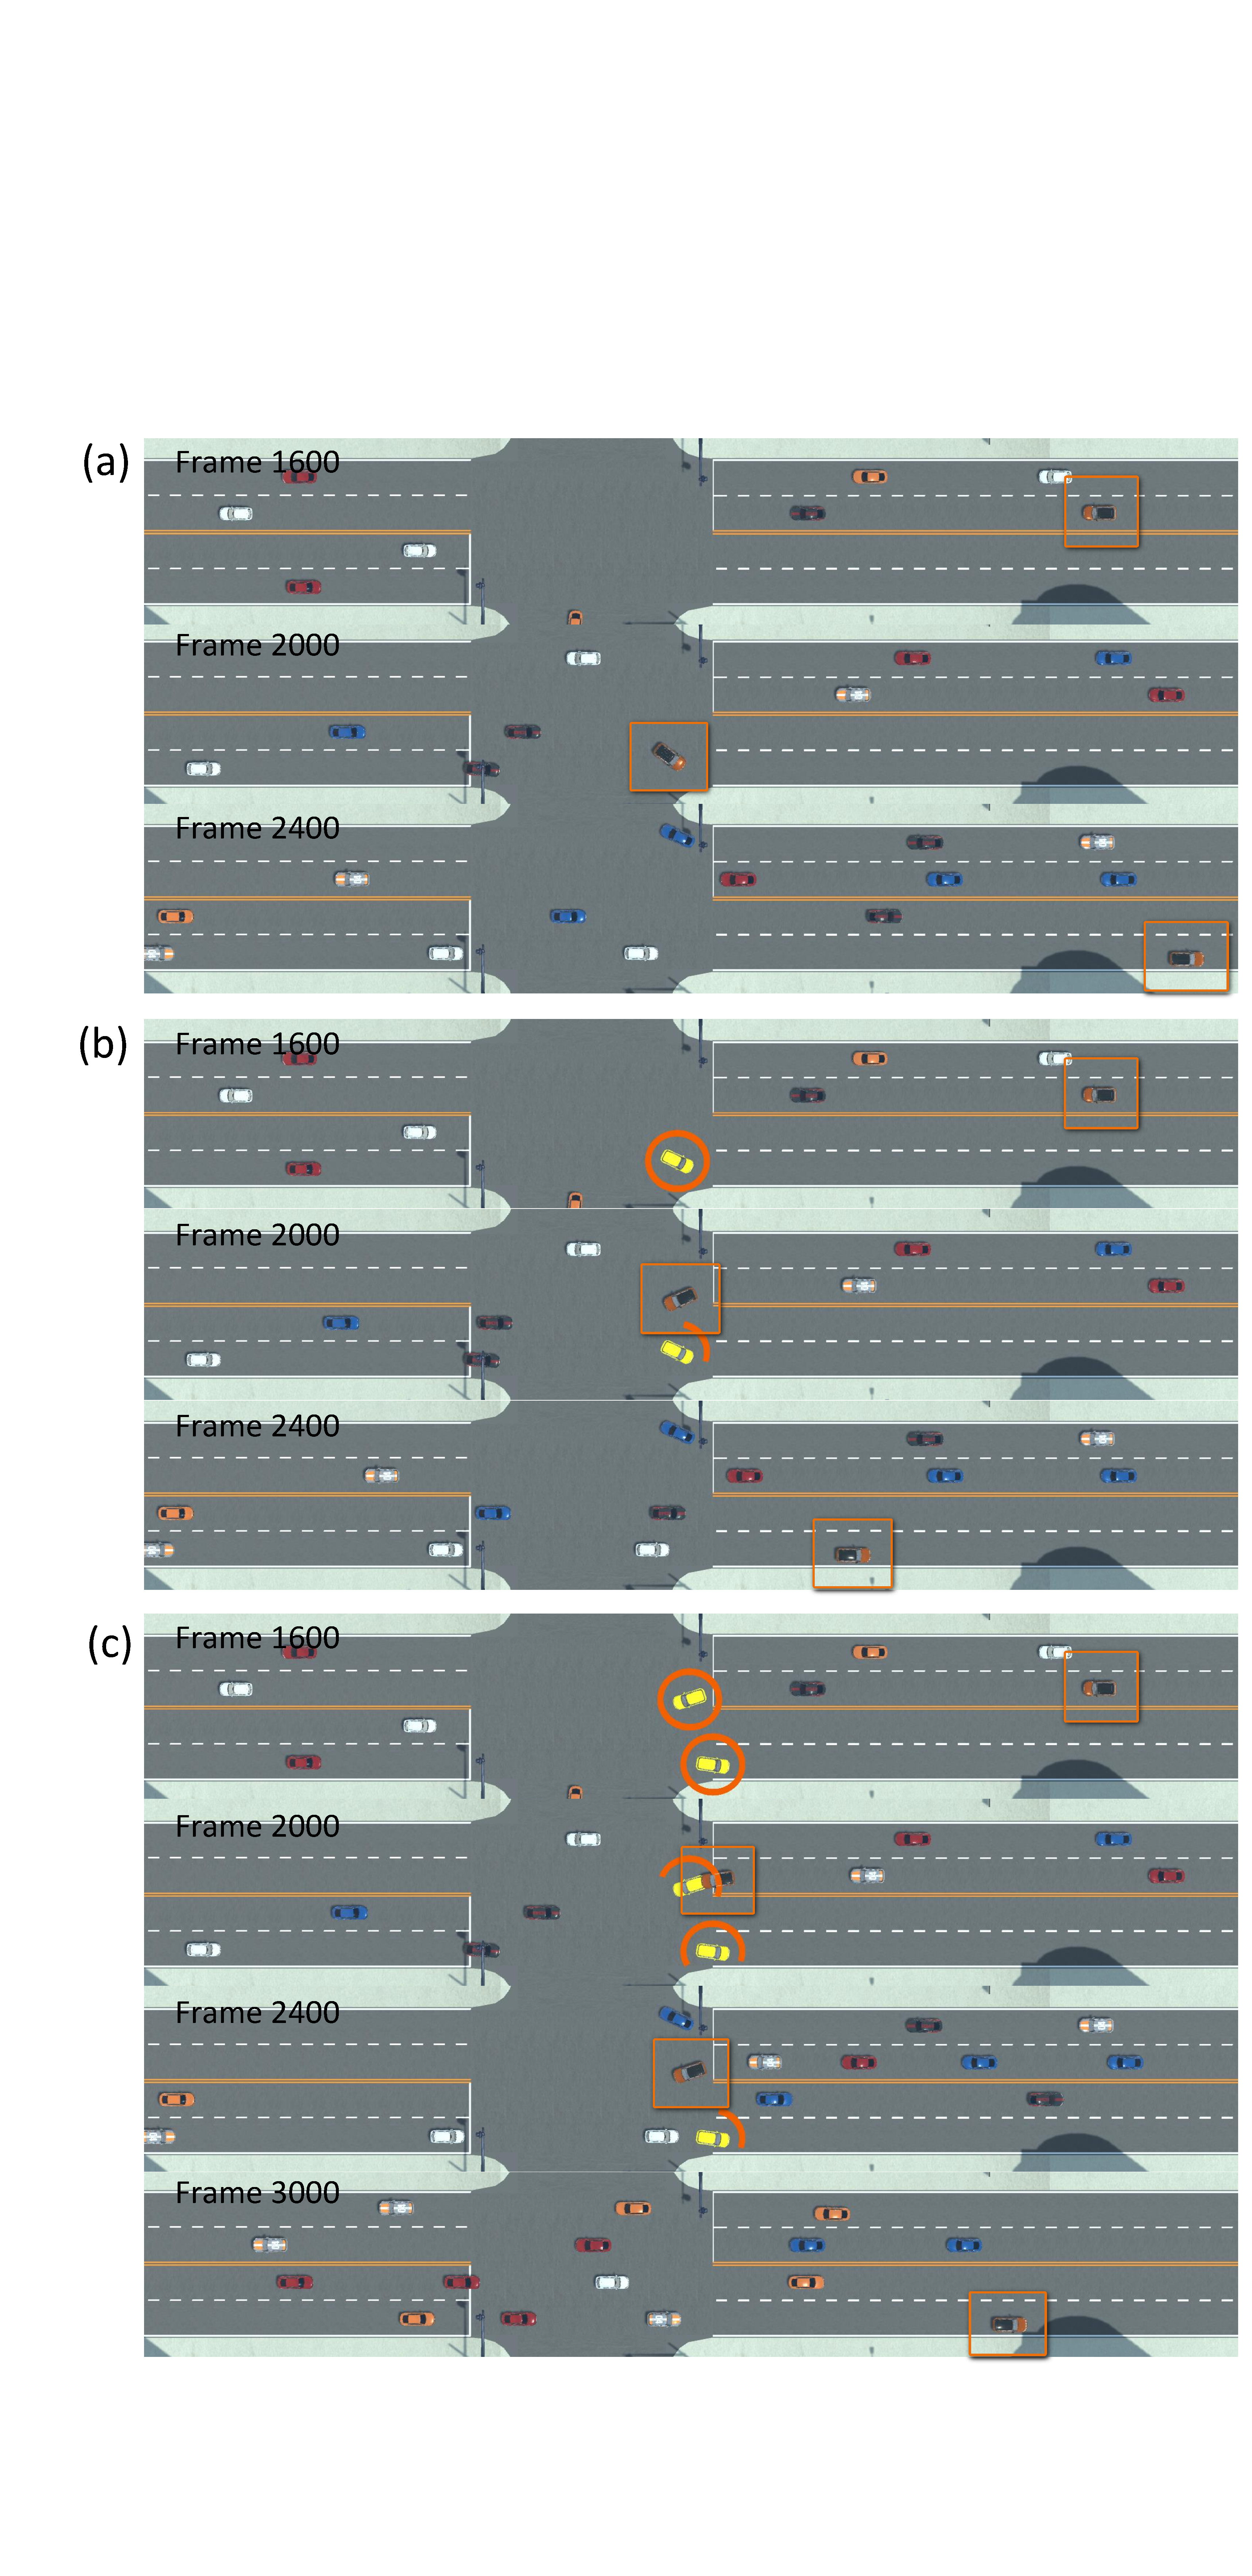
\includegraphics[width=0.78\textwidth]{figure/keyframe/failure_cases2_v3.pdf}
%\caption[因过弯异常而失败的案例与修复结果]{第二个失败案例。(a) 被编辑的车辆在进行U型掉头时保持了一个与实际不符的高速。(b) 第一个解决办法是赋予其另一个关键帧,使其在掉头之前减速而达到一个安全过弯速度。(c) 第二个解决办法是赋予其另两个关键帧,使其在掉头之前制动,等待对向来车先行通过后方才继续完成掉头,避免激进或不文明的驾驶行为。}
\caption[因过弯异常而失败的案例与两种修复结果]{
因过弯异常而失败的案例与两种修复结果
}
\label{fig:keyframe_failure2}
\end{figure}




\section{本章小结}

我们提出了一种新颖的交通轨迹编辑方法,允许用户指定时-空关键帧来控制车辆的行为,生成预期的交通轨迹。我们提出了一个基于社会力的交通仿真框架,同时考虑了车辆所受的自驱动力、路径保持力和碰撞避免力,且使用Cartesian坐标系和Frenet坐标系混合的方式来表示车辆的状态和更新车辆的行为。为了求解关键帧的约束控制,我们提出了一个由粗到细的优化过程。首先,我们沿着参考路径离散化的状态-时间空间,构建状态-时间图,并规划从起点到关键帧对应节点的粗粒度轨迹;然后,我们利用粗粒度轨迹中提取的信息来初始化伴随法,使梯度下降快速稳定地收敛,高效地找到一组最佳的控制预期速度,基于我们的社会力模型仿真生成更精细、平滑的轨迹。实验结果显示,我们的方法无论是在运动控制还是关键帧求解部分均能达到毫秒级别,因此可以给予用户实时的关键帧控制和个体运动变化反馈;而在面对一些单次交互无法处理的失败案例时,我们的方法也有能力支持用户进行迭代式的编辑修复,使最终结果不断趋近用户的预期。


本方法仍然存在一些限制。首先,如果仿真环境拥挤,被编辑车辆拥有大量的邻车,那么关键帧的约束可能会失效。正如我们在章节~\ref{section:keyframe_coarseopt}中所述,状态-时间搜索过程中会将邻车视为静态的障碍物,这意味着在优化过程中邻车并不会被同时调整,若车辆在状态-时间搜索规划轨迹时由于被阻挡而无法到达关键帧,我们会返回一条能到达最接近实际目标节点的轨迹。虽然该问题可以通过迭代地编辑目标车辆或邻车,但一个能一次性考虑所有车辆的优化过程同样是非常具有探索价值的。其次,由于用户的任意编辑,车辆的仿真行为有可能会变异常。例如,在真实的交通中,当车辆沿着弯道行驶时,为了安全和舒适驾驶员会提前减速,而并非保持高速行驶。这个问题同样也可以通过人为地添加更多关键帧和其他约束来解决,使得车辆的运动在视觉上更符合常理。
